\documentclass[titlepage]{article}
\usepackage[nouppercase]{frontespizio}

\usepackage{amsmath}
\usepackage[utf8]{inputenc}
\usepackage[italian]{babel}

\usepackage{pgfplots}
\pgfplotsset{compat=1.16}

\usepackage{graphicx}
\graphicspath{{./immagini/}}
\usepackage{hyperref}
\hypersetup{
    colorlinks=true,
    linkcolor=black,
    urlcolor=blue
}

% Impostazioni per i listati di codice:
\usepackage{xcolor}
\definecolor{background}{HTML}{F7F7F7}
\usepackage{minted}
\setminted[python]{
framesep=2mm,
baselinestretch=1.2,
bgcolor=background,
fontsize=\footnotesize,
breaklines=true,
linenos
}

% Tabelle:
\usepackage{booktabs}
\usepackage{makecell}
\usepackage{multirow}


\begin{document}

\begin{frontespizio}
\Universita{Verona}
\Dipartimento{Informatica}
\Scuola{CdLM in Ingegneria e scienze informatiche}
\Titolo{Authorship attribution}
\Sottotitolo{Progetto per il corso di Big Data}
\Candidato[VR464051]{Michele Dalla Chiara}
\Candidato[VR458470]{Davide Zampieri}
\Annoaccademico{2020-2021}
\NCandidati{}
\Punteggiatura{}
\end{frontespizio}

\tableofcontents
\newpage

\section{Introduzione}
\label{sec:1}
Questo documento rappresenta la relazione del progetto sulla \textit{authorship attribution} svolto nell'ambito del corso di Big Data della Laurea magistrale in Ingegneria e scienze informatiche presso l'Università di Verona.

\subsection{Etimologia della parola Big Data}
\textit{Big Data} è un termine molto conosciuto che è entrato prepotentemente nel vocabolario linguistico di molte persone. Come esempio di impiego dei Big Data possiamo citare i siti di e-commerce, i quali possono utilizzare i Big Data per proporre ad un utente determinati prodotti che potrebbero interessargli. Per fare ciò vengono raccolte inizialmente una serie di informazioni riguardanti il cliente, come ad esempio i prodotti ricercati o i prodotti precedentemente acquistati. Dopo aver raccolto tali informazioni, queste devono essere elaborate al fine di proporre i prodotti giusti al cliente.

In modo informale possiamo descrivere i Big Data come una massa di dati, anche eterogenei fra loro, che devono innanzitutto essere memorizzati per poi successivamente venire elaborati. Per raggiungere questi obiettivi, un solo calcolatore chiaramente non può essere sufficiente.

\subsection{Caratteristiche dei Big Data}
I Big Data verificano le seguenti \textit{caratteristiche}:
\begin{itemize}
    \item Volume.
    \item Velocity.
    \item Variety.
\end{itemize}
\begin{figure}[htp]
	\centering
	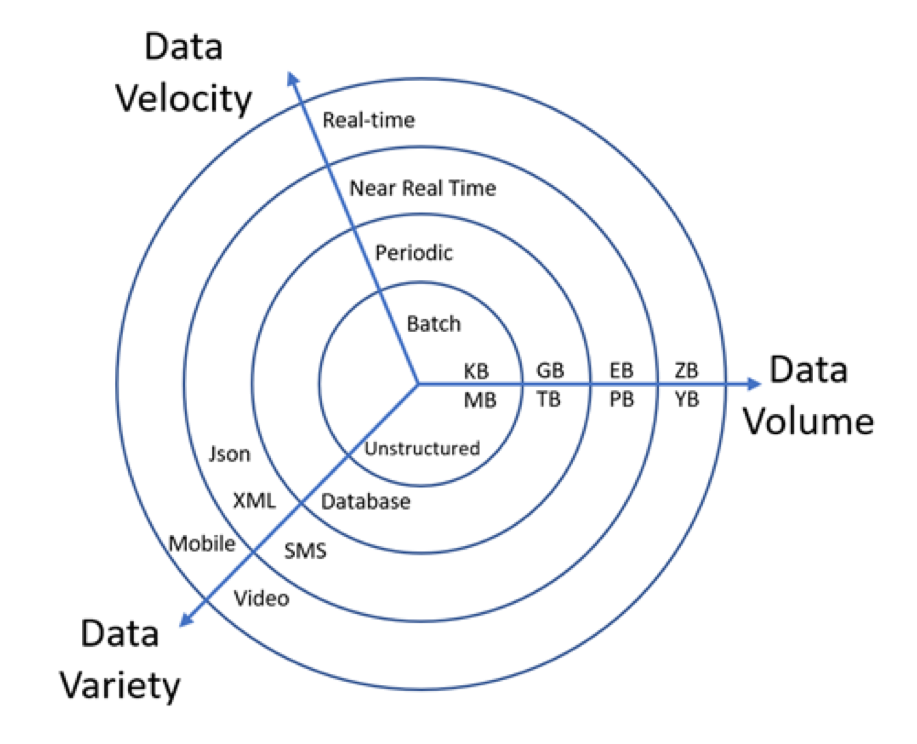
\includegraphics[width=0.65\textwidth]{3V.png}
\end{figure}

\textit{Volume} si riferisce alla quantità dei dati; in particolare, quando parliamo di Big Data l'ordine di grandezza può variare tra la decina di TeraByte e qualche PetaByte o ZetaByte. Per memorizzare masse così grandi di dati è necessario avere uno storage scalabile, ovvero dobbiamo in qualsiasi momento avere la possibilità di aggiungere nuovo storage a quello già esistente in modo semplice e trasparente.

\textit{Velocity} specifica non solo la velocità di produzione di nuovi dati ma anche la velocità, da parte di un client, di ottenere delle risposte. Questa è una caratteristica molto importante per gli e-commerce i quali, dopo aver raccolto i dati di navigazione di un consumatore, devono essere più rapidi nel suggerire prodotti di interesse per il cliente.

\textit{Variety} indica, infine, che esistono diversi modi in cui i dati arrivano al sistema di elaborazione dei Big Data. Infatti i dati, oltre ad essere di forma diversa, possono anche essere raccolti da dispositivi di  tipologia differente. Da questi dati non strutturati è importante estrarre delle informazioni, in modo da farli diventare dei dati strutturati.

\subsection{Scopo del progetto}
L'\textit{idea} del progetto deriva dal fatto che di tanto in tanto vengono ritrovati degli scritti anonimi che devono essere attribuiti a degli autori. In genere, questo compito viene svolto da persone esperte del settore che conoscono molto bene i diversi stili degli autori.

Lo \textit{scopo} del progetto è quello di creare un applicativo che analizzi testi di autori famosi per estrarne le caratteristiche stilistiche e, successivamente, permetta di sottoporre altri scritti cercando di \emph{stabilirne la paternità}. In pratica, il programma dovrà confrontare le caratteristiche estratte da un testo sconosciuto con quelle di autori ``noti'' (ossia quelli che il sistema ha imparato a riconoscere) al fine di identificare la persona che scrisse il testo sconosciuto.


\newpage
\section{Hadoop Map-Reduce vs Spark}
\label{sec:2}
Per la \textit{realizzazione} del progetto è stato impiegato il modello di programmazione Spark. \`{E} stato preferito rispetto a Map-Reduce di Hadoop poiché, nonostante Map-Reduce sia un framework molto popolare, è più rigido nello stile di programmazione rispetto a Spark; in più, Map-Reduce non dà la stessa possibilità di scelta di operatori che invece può offrire Spark.

\subsection{Cos'è Hadoop}
Circa una ventina di anni fa gli ingegneri si resero conto che scalare verso l'alto, ovvero aumentare le capacità di una singola macchina, non era sufficiente per gestire una sempre più grande mole di dati. Inoltre, i costi per scalare verso l'alto non erano proporzionali alla crescita della capacità della macchina; infatti la curva costi-capacità è di forma logaritmica. Proprio per questo motivo, nel 2005, nasce \textit{Hadoop}, un framework che permette la memorizzazione e l'elaborazione di dataset di grandi dimensioni usando una batteria (cluster) di calcolatori. Le componenti più importanti di Hadoop sono:
\begin{itemize}
    \item \textit{Hadoop common}, collezione di librerie e script necessari al funzionamento e alla gestione di Hadoop. È un elemento molto importante perché realizza un livello di astrazione che permette al programmatore di concentrarsi sull'applicativo e non su aspetti relativi ai problemi di rete o alla sincronizzazione/comunicazione tra processi ecc.
    \item \textit{YARN}, componente di Hadoop che separa la gestione delle risorse dalle componenti di elaborazione.
    \item \textit{HDFS}, filesystem distribuito usato per la gestione dei file presenti nello storage dei server che compongono il sistema distribuito su cui viene eseguito Hadoop.
    \item \textit{Map-Reduce}, framework software che si occupa di elaborare i job inviati dai client tramite un processo Map che genera delle coppie chiave/valore ed un processo Reduce che rielabora le coppie ricevute sulla base della loro chiave.
\end{itemize}

\subsubsection{Cluster}
Un principio importante legato al clustering è la scalabilità che deve avvenire in modo semplice e trasparente permettendo ad Hadoop di passare da qualche decina a diverse centinaia di server. Ogni calcolatore mette a disposizione le proprie risorse di elaborazione e memorizzazione. In generale, le capacità del sistema distribuito aumentano in relazione al numero di calcolatori tuttavia, i \textit{cluster} con tante macchine saranno maggiormente soggetti a guasti; se pensiamo che un computer possa guastarsi con una certa probabilità $p$, anche molto piccola, allora la probabilità che si guasti un cluster è data dal prodotto della probabilità di guasto di un elemento del cluster per il numero di elementi che lo compongono.

Hadoop rinuncia all'affidabilità per ottenere un sistema in grado di rilevare e gestire fallimenti a livello applicativo in modo da rendere il sistema sempre disponibile.

\subsubsection{Caratteristiche dell'HDFS}
HDFS (Hadoop Distributed File-System) ha importanti \textit{caratteristiche} che lo contraddistinguono dai suoi simili, ossia:
\begin{itemize}
    \item Un dato può essere letto tante volte ma scritto una volta sola.
    \item Non gestisce accessi concorrenti alla stesso blocco, ma permette la replicazione dei dati.
    \item In caso di guasti fornisce i servizi in modo trasparente (fault-tolerant).
    \item I dati di grandi dimensioni vengono divisi in \textit{blocchi} da 64 o 128 MB salvati anche su macchine diverse, permettendo dunque un accesso parallelizzato e più rapido.
\end{itemize}
Ogni nodo del sistema può essere un NameNode o un DataNode. In particolare, il NameNode è il nodo \textit{master} che gestisce uno o più nodi \textit{slave} (i DataNode).
\begin{figure}[htp]
	\centering
	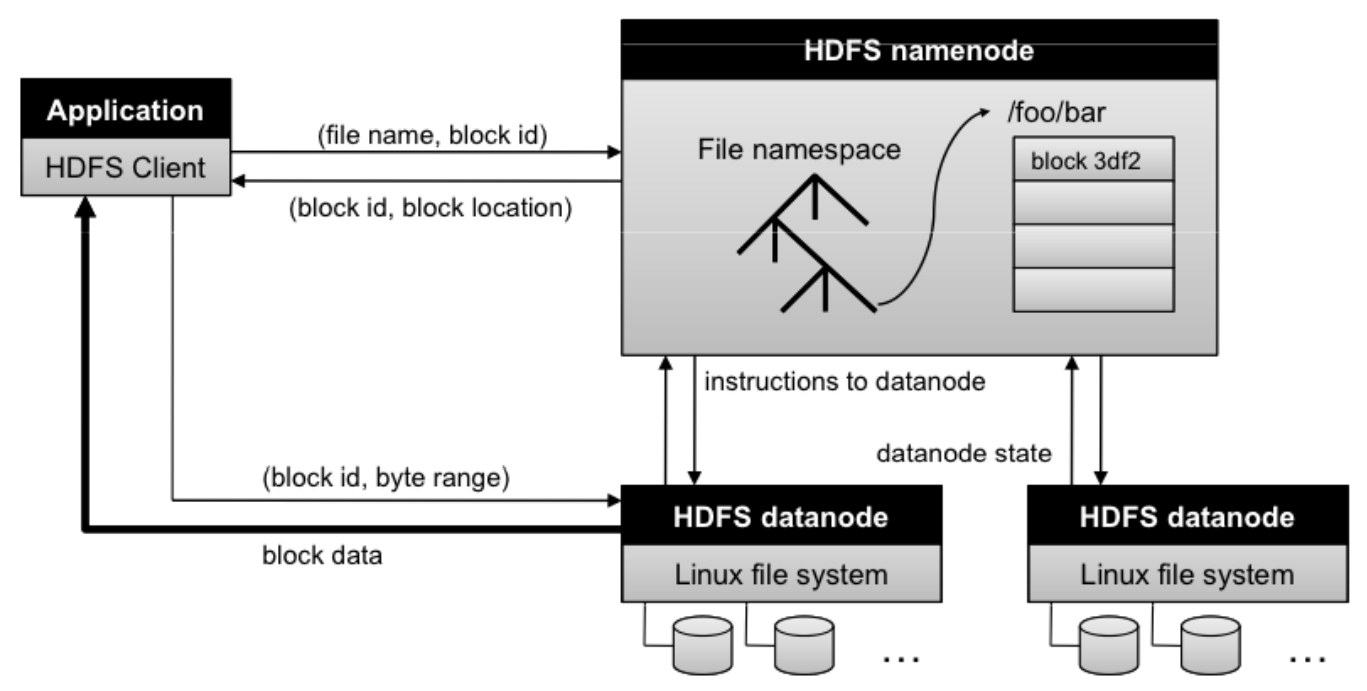
\includegraphics[width=0.7\textwidth]{nodi.png}
\end{figure}

Il \textit{NameNode} viene mantenuto in memoria RAM e contiene dei metadati; è una componente fondamentale perché senza di esso il filesystem non potrebbe funzionare. Nel NameNode si tiene traccia di quali blocchi vengono gestiti dal nodo e della posizione delle repliche (dei blocchi). Infine, viene mantenuta anche l'immagine dell'intero namespace del filesystem sempre su memoria RAM.

Il \textit{DataNode}, invece, è la collezione dei blocchi di dati mantenuti dal nodo; questa componente deve occuparsi di rispondere a eventuali richieste di accesso ai blocchi da parte dei client e deve anche inoltrare periodicamente al NameNode la lista dei blocchi gestiti.

Per esempio, nell'operazione di lettura il client interroga un NameNode per avere le informazioni sull'ubicazione dei blocchi di un file. Dopodiché il NameNode ritorna una lista, ordinata in base alla vicinanza al client, dei DataNode che contengono una copia del blocco richiesto.

\subsubsection{Paradigma Map-Reduce}
Map-Reduce è un paradigma di programmazione utilizzato in modo particolare da Hadoop per elaborare in maniera distribuita ed efficiente i Big Data. L'idea che ha portato alla nascita di questo paradigma è da ricercare nella programmazione funzionale. Il paradigma Map-Reduce in realtà si divide in 3 fasi:
\begin{enumerate}
    \item \textit{Map}, è la fase in cui si applica per ogni oggetto di un insieme, potenzialmente elaborato anche su macchine diverse, una funzione, in genere di filtraggio, e si scrivono su HDFS i risultati parziali sotto forma di coppie (chiave,valore).
    \item \textit{Shuffle}, è la fase in cui vengono recuperati i risultati parziali, vengono raggruppati in base alla chiave (oppure tramite una funzione definita dal programmatore) e infine ogni raggruppamento viene inoltrato a nodi di elaborazione diversi.
    \item \textit{Reduce}, è l'ultima fase ed è quella in cui ogni nodo elabora i diversi raggruppamenti per produrre un risultato da ciascuno di essi.
\end{enumerate}

\subsection{Cos'è Spark}
\textit{Spark} è un framework alternativo a Map-Reduce progettato per rendere più semplice e veloce la creazione e l'esecuzione di algoritmi che manipolano dati distribuiti. Spark risulta più veloce poiché è in grado di effettuare operazioni direttamente in memoria principale riuscendo ad offrire prestazioni anche 100 volte superiori rispetto alla controparte in Map-Reduce. Risulta più semplice da usare perché offre un insieme di primitive molto ampio semplificando di molto la programmazione. Spark può essere utilizzato con Java, Scala o Python. In particolare, per poter interagire con Spark in Python si usa l'API PySpark.

\subsubsection{Spark Driver e Spark Context}
Ogni applicazione Spark ha uno \textit{Spark Driver}, ovvero un programma che dichiara le operazioni da effettuare sulle RDD (spiegate nel dettaglio nella \hyperref[sec:2.2.2]{\textit{sezione 2.2.2}}) e che invia tali richieste al gestore del cluster. Le RDD rappresentano la principale astrazione della programmazione in Spark.

In realtà, il driver è il programma che crea \textit{Spark Context}, il quale poi creerà un job diviso in fasi ognuna delle quali a sua volta è suddivisa in task pianificate su un esecutore. Gli esecutori lanciano quindi il codice dell'utente eseguendo i calcoli ed, eventualmente, memorizzando nella cache vari dati utili all'applicazione. Quando si avvia PySpark, Spark Context viene creato e allocato automaticamente nella variabile \texttt{sc}. L'applicazione termina quando il driver viene chiuso mediante l'istruzione \texttt{sc.stop()}.
\begin{figure}[htp]
	\centering
	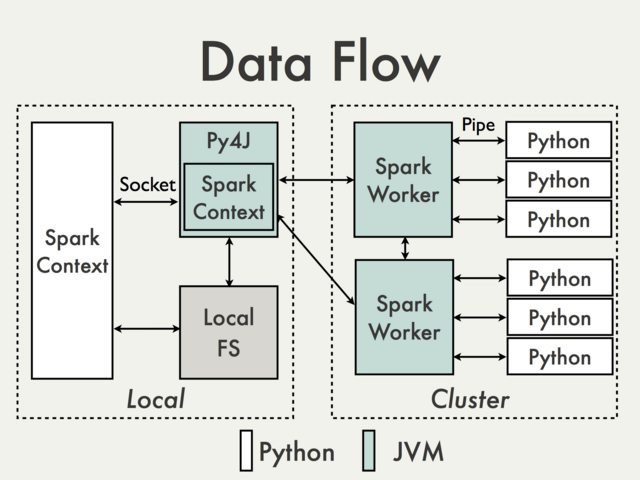
\includegraphics[width=0.7\textwidth]{data-flow.png}
\end{figure}

\subsubsection{Resilient Distributed Datasets (RDD)}
\label{sec:2.2.2}
Le RDD sono collezioni non modificabili di oggetti partizionati/distribuiti attraverso i nodi di un cluster che vengono archiviati nella memoria principale o eventualmente su disco locale. Una RDD può puntare a dei dati o applicare alcune operazioni (in parallelo) per generarne di nuovi.

In PySpark le RDD sono come le liste di Python, ovvero permettono di memorizzare oggetti di diverso tipo.

\subsubsection{Operazioni}
I programmi vengono scritti come composizione di operazioni sulle RDD. Le RDD vengono manipolate e costruite attraverso trasformazioni e azioni. Le \textit{trasformazioni} non sono eseguite nel momento in cui vengono richiamate (perché lavora in modalità lazy), bensì nulla viene eseguito fino a quando il driver non invoca un'\textit{azione}. Le trasformazioni si dividono in:
\begin{itemize}
    \item Trasformazioni \textit{narrow}, in cui ogni partizione della RDD genitore viene utilizzata da al massimo una partizione della RDD figlia. Fra le trasformazioni \textit{narrow} troviamo ad esempio: \texttt{map}, \texttt{flatMap}, \texttt{filter}, \texttt{sample}, \texttt{union}, ecc.
    
    \item Trasformazioni \textit{wide}, in cui più partizioni della RDD figlia possono dipendere dalla stessa partizione della RDD padre. Fra le trasformazioni \textit{wide} ci sono invece: \texttt{reduceByKey}, \texttt{groupByKey}, \texttt{join}, \texttt{repartition}, ecc.
\end{itemize}
\newpage
\begin{figure}[htp]
	\centering
	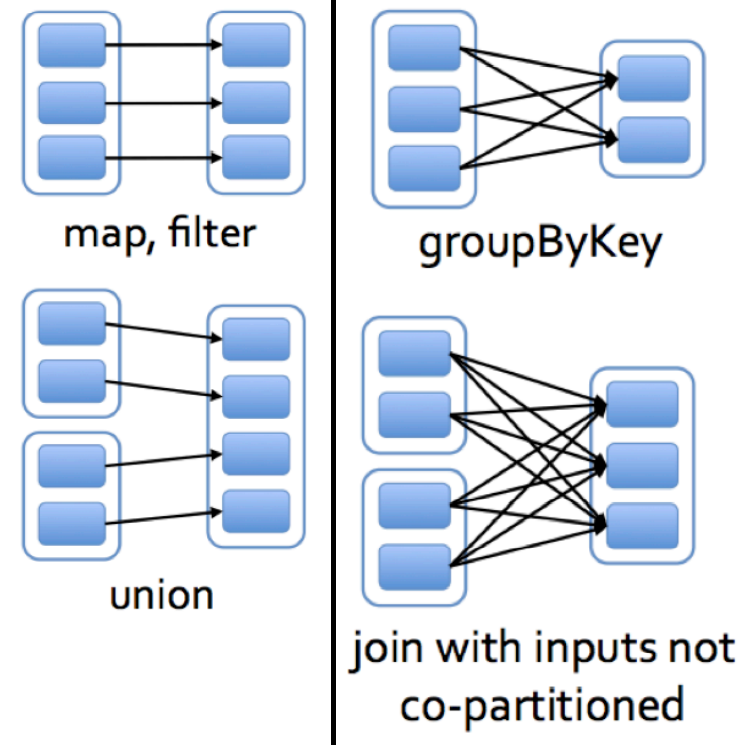
\includegraphics[width=0.7\textwidth]{trasformazioni.png}
\end{figure}

\noindent
Sono esempi di azioni:
\begin{itemize}
    \item \texttt{count}, \texttt{collect}, \texttt{take}, \texttt{top}, \texttt{saveAsTextFile}, ecc.
\end{itemize}


\newpage
\section{Struttura del progetto}
\label{sec:3}
Il progetto è stato diviso in più moduli i quali vengono richiamati da un programma main che controlla il flusso di lavoro dell'applicativo.

Il \textit{flusso di lavoro} generale (che non distingue fra testo sconosciuto e testo di training per il classificatore) lo possiamo rappresentare attraverso i seguenti punti:
\begin{enumerate}
    \item Caricamento dei testi.
    \item Calcolo delle caratteristiche di stile.
    \item Salvataggio delle caratteristiche di stile.
    \item Analisi di nuovi testi (ripetendo dal punto \emph{1}).
\end{enumerate}
Quando in input abbiamo dei testi sconosciuti, rispetto al flusso di lavoro descritto poc'anzi, troviamo chiaramente l'operazione di classificazione che è l'ultima ad essere eseguita e permette di stabilire, rispetto agli autori che il classificatore conosce, chi possa essere ad aver prodotto lo scritto.

\subsection{Riflessione sulla natura del classificatore}
\label{sec:3.1}
Per lo sviluppo dell'applicativo sono state impiegate conoscenze legate alla Machine Learning. Essa è una parte dell'intelligenza artificiale che ha come obiettivo quello di riuscire a determinare i parametri che minimizzano i potenziali errori di classificazione. In particolare noi abbiamo pensato di realizzare un classificatore Bayesiano. Il termine Bayesiano è legato al teorema su cui il classificatore si basa ovvero:
\begin{equation}
    p(C_i | x) = \frac{p(x | C_i) \cdot p(C_i)}{p(x)}
\end{equation}
dove $C_i$ è la classe i-esima e $x$ è un elemento di un dataset. Supponiamo di avere due classi $C_1$ e $C_2$. Dal teorema di Bayes riusciamo a ricavare la regola fondamentale nota come regola di decisione, la quale afferma che se $p(C_1 | x) > p(C_2 | x)$ allora etichettiamo $x$ come elemento della classe $C_1$ altrimenti della classe $C_2$. Questa scelta è la migliore che possiamo prendere in quanto se definiamo la probabilità d'errore come
\begin{equation}
    p(error | x) = \begin{cases}
    p(C_1 | x) & \text{se abbiamo scelto $C_2$} \\
    p(C_2 | x) & \text{se abbiamo scelto $C_1$}
    \end{cases}
\end{equation}
è chiaro che se prendiamo la probabilità $p(C_i | x)$ maggiore allora questa minimizza l'errore. 

Un aspetto molto importante in un processo di classificazione riguarda le dimensioni del cosiddetto spazio delle features, il quale non è altro che uno spazio matematico in cui ciascuna dimensione rappresenta una specifica feature (una riga di un vettore colonna) su cui andiamo a collocare gli elementi del nostro dataset.

\noindent
Matematicamente gli elementi possiamo definirli come vettori della forma
\begin{align}
    elemento &= \begin{bmatrix}
        x_{1} \\
        x_{2} \\
        \vdots \\
        x_{m}
        \end{bmatrix}
  \end{align}
con $m=|$\textit{spazio delle features}$|$.

Nel nostro caso, lo spazio delle features è dato da tutti gli attributi stilistici che riusciamo ad estrarre dai testi. Il numero totale di questi attributi è molto alto e per questo \emph{di solito} si tende a ridurre la dimensione dello spazio matematico attuando tecniche di feature extraction o feature selection, poiché se il numero di features è molto grande la nuvola di punti (che non sono altro che gli elementi del dataset) sarà molto sparsa e questo non va bene. Concretamente questo significa che se lo spazio delle features ha un numero di dimensioni molto elevato serve un dataset estremamente grande per permettere \emph{una buona taratura} dei parametri del classificatore.
\begin{figure}[htp]
	\centering
	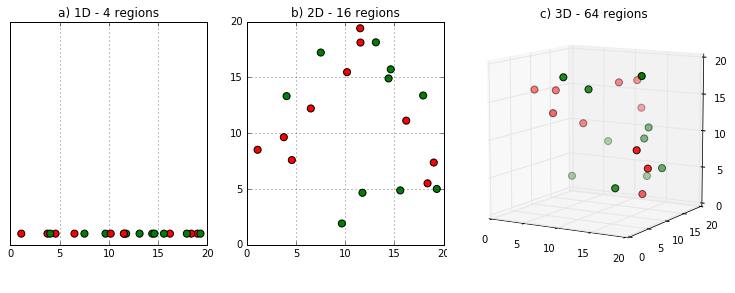
\includegraphics[width=\textwidth, height=\textheight, keepaspectratio]{curse-of-dimensionality.png}
\end{figure}

\noindent
Purtroppo noi non possiamo operare questa riduzione in quanto, trattando di authorship attribution, si evince che tutte le features devono essere considerate al fine di definire lo stile di un autore. A causa di questo aspetto e dell'elevato numero di dimensioni, per realizzare un classificatore Bayesiano puro è necessario avere a disposizione un dataset davvero molto grande. Tutto questo ci ha fatto riflettere e siamo giunti alla conclusione che per classificare fosse necessario considerare gli attributi separatamente e stabilire se un testo presenta l'attributo stilistico con una certa probabilità. Sommando queste probabilità e dividendo per il numero totale di attributi determiniamo la probabilità $p(Autore | x)$ che un testo sia stato scritto da un certo autore. Per ogni autore calcoliamo $p(Autore_i | x)$ e determiniamo la probabilità maggiore rispettando quindi la regola di decisione descritta precedentemente.

\subsection{Calcolo delle caratteristiche di stile}
Per lo \textit{spazio stilistico} di un autore si è deciso di utilizzare gli attributi presentati nella seguente tabella (in cui la colonna ``famiglia'' rappresenta i gruppi stilistici, la sigla SL indica la lunghezza di una frase e MCW è la sigla che indica la parola più comune).
\begin{center}
\begin{tabular}{cll}
    \toprule
    \textbf{FAMIGLIA} & \textbf{SIGLA} & \textbf{DESCRIZIONE} \\
    
    \midrule
    \multirow{4}{*}{\textit{Intero testo}} & V & Dimensione del vocabolario \\
    & T & Lunghezza del testo (numero di parole) \\
    & V/T & Rapporto fra V e T \\
    & H & Entropia \\
    
    \midrule
    \multirow{5}{*}{\textit{Frasi}} & MSL & Lunghezza massima di una frase \\
    & ASL & Lunghezza media di una frase \\
    & mSL & Lunghezza minima di una frase \\
    & PDSL & Distribuzione di probabilità delle SL \\
    & pMFSL & Probabilità della SL più frequente \\
    
    \midrule
    \multirow{5}{*}{\textit{Parole}} & PkMCW & Distribuzione di probabilità delle 30 MCW \\
    & pMCW & Probabilità della MCW (senza `and' e `the') \\
    & pMCWx & Probabilità della MCW (senza art. e prep.) \\
    & pThe & Probabilità della parola `the' \\
    & pComma & Probabilità della virgola \\
    
    \midrule
    \multirow{4}{*}{\textit{Distanze}} & \makecell[l]{adMCW,\\mdMCW,\\MsMCW} & \makecell[l]{Distanza media/minima/massima \\ tra apparenze consecutive della MCW} \\
    & \makecell[l]{adMCWx,\\mdMCWx,\\MsMCWx} & \makecell[l]{Distanza media/minima/massima \\ tra apparenze consecutive della MCW \\ escludendo articoli e preposizioni} \\
    & \makecell[l]{adThe,\\mdThe,\\MsThe} & \makecell[l]{Distanza media/minima/massima \\ tra apparenze consecutive di `the'}  \\
    & \makecell[l]{adComma,\\mdComma,\\MsComma} & \makecell[l]{Distanza media/minima/massima \\ tra apparenze consecutive della virgola} \\
    
    \bottomrule
\end{tabular}
\end{center}

\newpage
\subsubsection{Attributi sull'intero testo}
\paragraph{Funzione word\_counter.}
Per calcolare la \textit{dimensione del vocabolario} (ma non solo, come si vedrà più avanti) ci si serve della funzione \texttt{word\_counter} la quale, data una RDD che rappresenta un testo, conta quante volte compare ogni parola. Le trasformazioni usate in questa funzione sono:
\begin{itemize}
    \item \texttt{flatMap}, per trasformare una riga della RDD in un insieme di parole in modo che ogni parola sia un oggetto della nuova RDD.
    \item \texttt{map}, per trasformare ogni parola nella RDD in una tupla composta dalla parola stessa e dal valore 1.
    \item \texttt{reduceByKey}, per sommare tutte le frequenze della stessa parola ottenendo una RDD in cui ogni elemento è una tupla composta dalla parola e dalla relativa frequenza totale con cui essa appare all'interno del testo.
    \item \texttt{sortBy}, per ordinare le parole in base alla loro frequenza totale (in modo decrescente).
\end{itemize}
Infine, è stata usata l'azione \texttt{count} per attivare il conteggio del numero di elementi presenti nella RDD (dimensione del vocabolario).
\begin{minted}{python}
def word_counter(RDD):

    word_counter = (RDD.flatMap(lambda x: x)
                    .map(lambda x: (x,1))
                    .reduceByKey(lambda a,b: a+b)
                    .sortBy(lambda x: -x[1])
                   )
                   
    return word_counter, word_counter.count()
\end{minted}

\paragraph{Funzione text\_length\_in\_words.}
Per calcolare la \textit{lunghezza del testo} in termini di numero di parole si parte dalla RDD restituita dal word count e si eseguono le seguenti trasformazioni:
\begin{itemize}
    \item \texttt{map}, per tenere solamente tutte le frequenze totali delle varie parole (passando da coppie chiave/valore a singoli valori).
    \item \texttt{reduce}, per sommare tra loro tutti i valori presenti nella RDD (ossia le frequenze totali).
\end{itemize}
\begin{minted}{python}
def text_length_in_words(RDD_word_counter):

    return (RDD_word_counter.map(lambda x: x[1])
            .reduce(lambda a,b: a+b)
           )
\end{minted}

\paragraph{Funzione entropy.}
Per determinare l'\textit{entropia}, ossia il numero medio di bit richiesti per rappresentare tutte le parole di un testo, si calcola la seguente formula
\[ H(X) = - \sum_{x \in X} p(x) \cdot \log_2 p(x) \]
dove $x$ è una parola del testo $X$. Tramite l'uso delle trasformazioni \texttt{map} e \texttt{reduce} a partire dalla RDD restituita dal word count e dalla lunghezza del testo (utile per riuscire a calcolare le probabilità delle varie parole) riusciamo a determinare l'entropia di tale testo.
\begin{minted}{python}
def entropy(RDD_word_counter, text_len):

    return -(RDD_word_counter.map(lambda x: (x[1]/text_len) * math.log2(x[1]/text_len))
             .reduce(lambda a,b: a+b)
            ) # l'entropia ha segno negativo
\end{minted}

\subsubsection{Attributi sulle frasi}
\paragraph{Funzione sentence\_lengths.}
Questa funzione calcola le lunghezze (in termini di numero di parole) di tutte le frasi di un testo preso in input sotto forma di RDD. Come output viene restituita una nuova RDD contenente le \textit{lunghezze delle frasi}. Per individuare correttamente le frasi, è necessario effettuare le seguenti operazioni sul testo:
\begin{itemize}
    \item \texttt{flatMap} e \texttt{reduce}, per trasformare il contenuto della RDD in input in una stringa unica.
    \item Sostituzione dei caratteri \texttt{?} e \texttt{!} con il carattere \texttt{.} per identificare più facilmente i terminatori di una frase.
    \item Suddivisione della stringa quando si trova la terminazione di una frase (carattere \texttt{.} seguito da uno spazio).
\end{itemize}
Per calcolare le lunghezze delle frasi, invece, sono state usate le operazioni:
\begin{itemize}
    \item \texttt{parallelize}, per parallelizzare la stringa risultante dalle operazioni precedenti; tale stringa viene usata per formare un set di dati distribuito che può poi essere utilizzato in parallelo.
    \item \texttt{map}, per trasformare ogni frase considerata nel numero di parole che la compongono.
\end{itemize}
Grazie a quest'ultima trasformazione sarà poi possibile calcolare la lunghezza della frase massima, minima e media.
\begin{minted}{python}
def sentence_lengths(RDD):

    # operazioni preliminari sul testo
    text = RDD.flatMap(lambda x: x).reduce(lambda a,b: a + ' ' + b) # metto tutto il testo in una stringa unica
    text = text.replace("?", ".") # ? termina una frase
    text = text.replace("!", ".") # ! termina una frase
    text = text.split('. ') # split quando trovo un carattere che termina una frase (. seguito da uno spazio)
    
    return (sc.parallelize(text)
            .map(lambda x: len(x.split(' ')))
           ) # per ogni frase trovata conto le sue parole
\end{minted}

\paragraph{Funzione prob\_distr\_of\_sentence\_length.}
Per formare la distribuzione di probabilità delle lunghezze delle frasi si parte dalla RDD dell'output della funzione \texttt{sentence\_lengths} e si eseguono le seguenti trasformazioni:
\begin{itemize}
    \item \texttt{map}, per trasformare ogni lunghezza di frase nella RDD in una tupla della forma \textit{(lunghezza frase, 1)}.
    \item \texttt{reduceByKey}, per sommare tutti gli \textit{1} della stessa lunghezza ottenendo coppie composte da una lunghezza di frase e dalla relativa frequenza totale.
    \item \texttt{map}, per dividere ogni frequenza totale per il numero totale di frasi presenti nel testo (quest'ultimo numero si ottiene applicando l'azione \texttt{count} alla RDD originale per attivare il conteggio degli elementi che la compongono).
    \item \texttt{sortBy}, per ordinare (in modo decrescente) le lunghezze delle frasi in base alla loro probabilità di trovarsi nel testo.
\end{itemize}
\begin{minted}{python}
def prob_distr_of_sentence_length(RDD_sen_len):
    
    tot = RDD_sen_len.count()

    return (RDD_sen_len.map(lambda x: (x,1))
            .reduceByKey(lambda a,b: a+b)
            .map(lambda x: (x[0], x[1]/tot))
            .sortBy(lambda x: -x[1])
           )
\end{minted}

\newpage
\subsubsection{Attributi sulla probabilità delle parole}
\paragraph{Funzione prob\_distr\_of\_most\_common\_words.}
Per formare la distribuzione di probabilità delle parole più comuni si parte dalla RDD restituita dalla funzione \texttt{word\_counter} e si esegue la trasformazione \texttt{map} per dividere le frequenze di ogni parola presenti nella RDD per il numero totale di parole presenti nel testo (quest'ultimo numero viene passato in input come parametro della funzione e corrisponde alla lunghezza del testo calcolata dalla funzione \texttt{text\_length\_in\_words}).
\begin{minted}{python}
def prob_distr_of_most_common_words(RDD_word_counter, text_len):
    
    return RDD_word_counter.map(lambda x: (x[0], x[1]/text_len))
\end{minted}

\paragraph{Funzione prob\_of\_the\_most\_common\_word.}
La funzione ritorna la probabilità della parola più comune non considerando ``and'' e ``the'', in quanto queste ultime sono parole molto comuni nella lingua inglese ma sono poco significative per l'analisi delle caratteristiche di stile di un autore. Riguardo alle operazioni Spark, si parte dalla RDD contenente la distribuzione di probabilità delle parole più comuni e si eseguono:
\begin{itemize}
    \item \texttt{filter}, per selezionare le coppie della forma \textit{(parola, probabilità)} che soddisfano una condizione booleana in cui si controlla che \textit{parola} sia diversa da ``and'' e ``the''.
    \item \texttt{take(1)}, per restituire un array che contiene il primo elemento della RDD risultante dalla trasformazione precedente.
\end{itemize}
La funzione ritorna poi in output una tupla, l'unica presente nell'array risultante dall'azione precedente, che rappresenta la MCW (Most Common Word) e la relativa probabilità.
\begin{minted}{python}
def prob_of_the_most_common_word(RDD_prob_distr_of_MCWs):

    return (RDD_prob_distr_of_MCWs
            .filter(lambda x: x[0] != "and" and x[0] != "the")
            .take(1)
           )[0]
\end{minted}

\paragraph{Funzione prob\_of\_the\_most\_common\_word\_x.}
La sigla MCWx identifica la parola più comune escludendo articoli e preposizioni in quanto poco significativi per identificare lo stile di un autore. Per calcolare la probabilità di MCWx consideriamo la RDD contenente la distribuzione di probabilità delle parole più comuni e, durante il filtraggio, controlliamo che \textit{parola} (il primo elemento delle coppie della forma \textit{(parola, probabilità)} presenti nella RDD) non appartenga alla lista di articoli e preposizioni della lingua inglese.

Viene ritornata una tupla, l'unica presente nell'array risultante dall'azione \texttt{take(1)}, che rappresenta la MCWx (Most Common Word tolti articoli e proposizioni) e la relativa probabilità.
\begin{minted}{python}
def prob_of_the_most_common_word_x(RDD_prob_distr_of_MCWs):
    
    prep_art_file = os.path.join(os.path.abspath(os.path.dirname(__file__)), 'prep_art.txt')
    prep_art = open(prep_art_file).read().splitlines()
    
    return (RDD_prob_distr_of_MCWs
            .filter(lambda x: x[0] not in prep_art)
            .take(1)
           )[0]
\end{minted}

\paragraph{Funzione prob\_of\_The.}
Il comportamento è uguale alle 2 funzioni precedenti con l'unica differenza che il filtraggio seleziona solamente la parola ``the''. Ritorna poi in output una tupla, l'unica presente nell'array risultante dall'azione \texttt{take(1)}, che rappresenta la parola ``the'' e la relativa probabilità.
\begin{minted}{python}
def prob_of_The(RDD_prob_distr_of_MCWs):
    
    return (RDD_prob_distr_of_MCWs
            .filter(lambda x: x[0] == "the")
            .take(1)
           )[0]
\end{minted}

\paragraph{Funzione prob\_of\_comma.}
Viene calcolata la probabilità di comparsa della virgola nel testo come rapporto tra il numero di parole che come ultimo carattere hanno la virgola (in un testo ben formato la virgola viene distanziata con uno spazio bianco solamente dalla parola alla sua destra) e il numero di parole totali. Per calcolarlo si parte dalla RDD contenente tutte le frasi di un testo (passata come parametro) e si eseguono le seguenti operazioni:
\begin{itemize}
    \item \texttt{flatMap}, per trasformare una riga della RDD in un insieme di parole (comprensive anche dei segni di punteggiatura) in modo che ogni parola sia un oggetto della nuova RDD.
    \item \texttt{filter}, per selezionare le parole che soddisfano la condizione booleana in cui si controlla che esse abbiano come ultimo carattere la virgola.
    \item \texttt{count}, per attivare il conteggio del numero di elementi presenti nella RDD risultante dalla trasformazione precedente così da ottenere le occorrenze totali della virgola nel testo in esame.
\end{itemize}
La funzione ritorna come risultato la divisione tra il numero ottenuto da \texttt{count} e la lunghezza del testo (passata come parametro alla funzione).
\begin{minted}{python}
def prob_of_comma(RDD_sentences_data, text_len):

    return (RDD_sentences_data
            .flatMap(lambda x: x)
            .filter(lambda x: "," in x)
            .count()
           ) / text_len
\end{minted}

\subsubsection{Attributi sulla distanza delle parole}
\paragraph{Funzione distance\_consec\_appear.}
Viene ritornata una lista che contiene le distanze tra occorrenze successive di una parola \texttt{word} passata come parametro alla funzione. La funzione è stata realizzata per essere il più generale possibile, per questo si può usare \texttt{distance\_consec\_appear} per calcolare anche la distanza fra due virgole consecutive. Si parte dalla RDD contenente tutte le frasi di un determinato testo per poi eseguire come trasformazioni:
\begin{itemize}
    \item \texttt{flatMap}, per avere un'unica collezione che contiene tutte le parole del testo invece di avere una collezione di collezioni di parole.
    \item \texttt{zipWithIndex}, per associare ad ogni parola nella RDD un indice che incrementa di una unità parola dopo parola; in questo modo riusciamo ad avere una lista di coppie della forma \textit{(parola, indice)}.
    \item \texttt{filter}, per rimuovere tutte le parole diverse da \texttt{word} o, nel caso in cui \texttt{word} sia la virgola, controllare se la stringa \texttt{','} appartiene al primo elemento di ogni coppia (questo perché i testi sono scritti ad esempio come ``word1, word2, word3'' e quindi la virgola fa parte delle parole ``word1,'' e ``word2,'').
    \item \texttt{map}, per proiettare solo le posizioni (indici) delle parole.
\end{itemize}
Dopo aver eseguito le trasformazioni, attraverso l'azione \texttt{collect} viene recuperata la lista avente tutte le posizioni nel testo della parola \texttt{word}. E alla fine di tutto questo viene calcolata la differenza fra due numeri consecutivi della lista riuscendo così a determinare la distanza (in termini di numero di parole) fra due \texttt{word} successive.

\begin{minted}{python}
def distance_consec_appear(RDD, word):
    
    if word == ',':
        vect_pos = (RDD.flatMap(lambda x:x)
                    .zipWithIndex()
                    .filter(lambda x: ',' in x[0])
                    .map(lambda x: x[1])
                    .collect()
                   )
    else:
        vect_pos = (RDD.flatMap(lambda x:x)
                    .zipWithIndex()
                    .filter(lambda x: x[0] == word)
                    .map(lambda x: x[1])
                    .collect()
                   )
    
    vect_dis = []
    for i in range(1, len(vect_pos)):
        vect_dis.append(vect_pos[i] - vect_pos[i-1])
    
    return vect_dis
\end{minted}

\subsection{Caricamento dei testi}
In questa sezione troviamo due funzioni che vengono usate per normalizzare le frasi degli scritti trasformandole in minuscolo e  rimuovendo quei caratteri che si ritengono inutili. Sono presenti inoltre le funzioni necessarie per caricare i testi nelle RDD.

\paragraph{Funzione remove\_number\_some\_punctuation\_marks.}
Vengono trasformate le stringhe in lowercase e vengono rimossi: i caratteri numerici, il carattere \texttt{"} e il carattere \texttt{--} (presente in molti testi).
\begin{minted}{python}
def remove_number_some_punctuation_marks(row):
    
    lowercase = row.lower()
    lowercase = lowercase.replace("--", " ")
    
    res = ""
    for char in lowercase:
        if not ('0' <= char <= '9' or char == '"'):
            res += char

    return res
\end{minted}

\paragraph{Funzione remove\_number\_punctuation\_marks.}
Dopo aver cambiato in lowercase le frasi vengono eliminati quei caratteri che non sono alfabetici come numeri e segni di punteggiatura (\texttt{,} oppure \texttt{?} eccetera); sono mantenuti solamente l'apostrofo e il trattino per gestire le parole composte.
\begin{minted}{python}
def remove_number_punctuation_marks(row):
    
    lowercase = row.lower()
    lowercase = lowercase.replace("--", " ")
    
    res = ""
    
    for char in lowercase:
        if 'a' <= char <= 'z' or char == ' ' or char == '-' or char == "'":
            res += char

    return res
\end{minted}

\paragraph{Funzione load\_file\_without\_punctuations\_marks.}
Carica un testo, presente in un file, in una RDD ritornando frasi che rispettano i criteri della funzione \texttt{remove\_number\_punctuation\_marks} sopra definita. Le trasformazioni effettuate sono:
\begin{itemize}
    \item \texttt{filter}, per mantenere solo stringhe diverse da \texttt{""} (stringa vuota) che sono false per il filtro.
    \item \texttt{map}, per applicare la funzione \texttt{remove\_number\_punctuation\_marks} ad ogni riga del testo. 
    \item \texttt{map}, le righe possono contenere più spazi bianchi; per questo motivo si divide la stringa con \texttt{split} e si esegue subito dopo un \texttt{join} per unire con \emph{un unico} spazio bianco la lista di parole ottenuta dal metodo \texttt{split}.
    \item \texttt{map}, ogni riga viene infine divisa in parole usando nuovamente \texttt{split}.
\end{itemize}
Nota: la penultima trasformazione potrebbe sembrare inutile, tuttavia applicare uno \texttt{split} su stringhe con più spazi bianchi consecutivi genererebbe una lista contenente anche stringhe vuote che verrebbero contate, come normali parole, dalla funzione \texttt{word\_counter}.
\begin{minted}{python}
def load_file_without_punctuations_marks(filepath):
    # caricamento del dataset
    raw_text = sc.textFile(filepath)

    # rimuoviamo i numeri e i segni di punteggiatura
    return (raw_text.filter(bool)            # rimuoviamo le stringhe vuote
        .map(remove_number_punctuation_marks)
        .map(lambda x : ' '.join(x.split())) # rimuoviamo diversi spazi bianchi
        .map(lambda row : row.split(" "))
       )
\end{minted}

\paragraph{Funzione load\_file\_without\_number.}
Questa funzione è gemella della funzione \texttt{load\_file\_without\_punctuations\_marks}. Le trasformazioni eseguite sono le stesse di quest'ultima funzione tuttavia, invece di impiegare la funzione \texttt{remove\_number\_punctuation\_marks}, nel primo \texttt{map} abbiamo utilizzato la funzione \texttt{remove\_number\_some\_punctuation\_marks} che toglie tutti i simboli che non sono alfabetici.
\begin{minted}{python}
def load_file_without_number(filepath):
    
    # caricamento del dataset
    raw_text = sc.textFile(filepath)

    # rimuoviamo i numeri e i segni di punteggiatura
    return (raw_text.filter(bool)            # rimuoviamo le stringhe vuote
        .map(remove_number_some_punctuation_marks)
        .map(lambda x : ' '.join(x.split())) # rimuoviamo diversi spazi bianchi
        .map(lambda row : row.split(" "))
       )
\end{minted}

\subsection{Salvataggio delle caratteristiche di stile}
A questo punto ci occuperemo di descrivere come viene prodotto il dizionario delle proprietà stilistiche di un testo e come questo possa essere caricato o salvato in memoria secondaria.

\paragraph{Funzione generate\_metrics.}
La funzione è estremamente complessa e lunga in quanto impiega molte procedure presentate nelle sezioni precedenti. Per questo motivo riassumiamo l'esecuzione evidenziando i punti più importanti:
\begin{enumerate}
    \item Si inizializza a vuoto il dizionario \texttt{res} che verrà ritornato.
    \item Viene usata \texttt{load\_file\_without\_punctuations\_marks} per ignorare i segni di punteggiatura presenti nelle frasi del testo da analizzare; con \texttt{persist()} viene mantenuta la RDD risultante nella memoria cache.
    \item Vengono calcolate e memorizzate tutte le caratteristiche stilistiche (attributi) che non richiedono segni di punteggiatura.
    \item Viene usata la funzione \texttt{load\_file\_without\_number} per mantenere i segni di punteggiatura ed eliminare i caratteri numerici.
    \item Vengono calcolate e memorizzate tutte le metriche che dipendono dai segni di punteggiatura.
    \item Viene popolato il dizionario \texttt{res} in modo che la chiave rappresenti il nome dell'attributo stilistico e il valore sia il risultato delle funzioni applicate ai punti \textit{3} e \textit{5}.
\end{enumerate}
\begin{minted}{python}
def generate_metrics(file_in):
    res = {}
    
    # consideriamo il testo SENZA i segni di punteggiatura
    print("Caricamento del file in memoria ...", end=" ")
    data = load_file_without_punctuations_marks(file_in)
    data.persist()
    print("caricamento completato")

    # calcoliamo le prime metriche
    print("Calcolo delle prime metriche, attendere ...", end=" ")
    RDD_word_counter, vocabulary_size = word_counter(data)
    RDD_word_counter.persist()
    text_length = text_length_in_words(RDD_word_counter)
    entropy_value = entropy(RDD_word_counter, text_length)
    
    RDD_prob_distr_of_MCWs = prob_distr_of_most_common_words(RDD_word_counter, text_length)
    prob_the_most_common_word = prob_of_the_most_common_word(RDD_prob_distr_of_MCWs)
    prob_the_most_common_word_x = prob_of_the_most_common_word_x(RDD_prob_distr_of_MCWs)
    prob_the = prob_of_The(RDD_prob_distr_of_MCWs)

    MCW = prob_the_most_common_word[0]
    dist_consec_MCW = distance_consec_appear(data, MCW)
    
    MCWx = prob_the_most_common_word_x[0]
    dist_consec_MCWx = distance_consec_appear(data, MCWx)
    
    dist_consec_the = distance_consec_appear(data, 'the')
    print("calcolo completato")

    # consideriamo il testo CON i segni di punteggiatura
    print("Caricamento del file in memoria ...", end=" ")
    sentences_data = load_file_without_number(file_in)
    sentences_data.persist()
    print("caricamento completato")
    
    # calcoliamo altre metriche
    print("Calcolo di ulteriori metriche, attendere ...", end=" ")
    RDD_sen_lengths = sentence_lengths(sentences_data)
    RDD_sen_lengths.persist()

    sen_lengths = RDD_sen_lengths.collect()

    prob_distr_freq_sen = prob_distr_of_sentence_length(RDD_sen_lengths)

    p_comma = prob_of_comma(sentences_data, text_length)

    dist_consec_comma = distance_consec_appear(sentences_data, ',')
    print("calcolo completato")
    
    # popoliamo il dizionario
    # attributi sull'intero testo
    res['vocabulary_size'] = vocabulary_size
    res['text_length'] = text_length
    res['V_T'] = vocabulary_size/text_length
    res['entropy'] = entropy_value
    
    # attributi sulle frasi
    res['avg_sentence_len'] = sum(sen_lengths)/len(sen_lengths)
    res['max_sentence_len'] = max(sen_lengths)
    res['min_sentence_len'] = min(sen_lengths)
    res['prob_distr_freq_sen'] = prob_distr_freq_sen.collect()
    res['prob_most_freq_sen'] = prob_distr_freq_sen.collect()[0][1]
    
    # attributi sulla probabilità delle parole
    res['prob_distr_of_30'] = RDD_prob_distr_of_MCWs.take(30)
    res['prob_of_the_most_common_word'] = prob_the_most_common_word[1]
    res['prob_of_the_most_common_word_x'] = prob_the_most_common_word_x[1]
    res['prob_of_the'] = prob_the[1]
    res['prob_of_comma'] = p_comma
    
    # attributi sulla distanza
    res['avg_dist_consec_comma'] = sum(dist_consec_comma)/len(dist_consec_comma)
    res['min_dist_consec_comma'] = min(dist_consec_comma)
    res['max_dist_consec_comma'] = max(dist_consec_comma)
    
    res['avg_dist_consec_MCW'] = sum(dist_consec_MCW)/len(dist_consec_MCW)
    res['min_dist_consec_MCW'] = min(dist_consec_MCW)
    res['max_dist_consec_MCW'] = max(dist_consec_MCW)
    
    res['avg_dist_consec_MCWx'] = sum(dist_consec_MCWx)/len(dist_consec_MCWx)
    res['min_dist_consec_MCWx'] = min(dist_consec_MCWx)
    res['max_dist_consec_MCWx'] = max(dist_consec_MCWx)
    
    res['avg_dist_consec_the'] = sum(dist_consec_the)/len(dist_consec_the)
    res['min_dist_consec_the'] = min(dist_consec_the)
    res['max_dist_consec_the'] = max(dist_consec_the)
    
    return res
\end{minted}

\subsubsection{Funzioni per salvare e caricare oggetti Python}
Per realizzare uno strumento che sia il più automatizzabile possibile, abbiamo implementato delle funzioni che permettono di caricare e salvare in un file di tipo binario i dizionari Python contenenti le caratteristiche di stile estratte da un testo di un determinato autore. Siccome tali file ``autore'' possono poi crescere nel tempo è stato deciso di salvarli direttamente sul filesystem HDFS. Per riuscire in tutto questo abbiamo usato le librerie \texttt{pickle} e \texttt{hdfs}. Quest'ultima permette infatti di aprire una connessione con l'ambiente distribuito in cui è presente il filesystem HDFS (nel nostro caso Cloudera) per poter poi effettuare le classiche operazioni di lettura e scrittura di file.

\paragraph{Funzione save\_metrics.}
Questa funzione permette di salvare il dizionario del testo specificato nel percorso \texttt{file\_in} in un file ``autore'' di destinazione chiamato \texttt{file\_out} (entrambi i percorsi vengono passati in input). I file ``autore'' contengono una lista di dizionari e questo dà la possibilità di estendere la lista aggiungendo nuove informazioni riguardanti gli autori.

La funzione crea inizialmente, attraverso \texttt{generate\_metrics}, il dizionario delle metriche; poi apre il file ``autore'' in modalità \textit{append} per salvare la struttura dati attraverso la funzione \texttt{dump} di \texttt{pickle}. Il blocco \texttt{try-except} serve ad assicurare che il file venga creato se non esiste.
\begin{minted}{python}
def save_metrics(file_in, file_out):

    entry = generate_metrics(file_in)
    
    client = InsecureClient('http://quickstart.cloudera:50070')
    try:
        with client.write(file_out, append=True) as fout:
            pickle.dump(entry, fout, pickle.HIGHEST_PROTOCOL)
    except:
        with client.write(file_out) as fout:
            pickle.dump(entry, fout, pickle.HIGHEST_PROTOCOL)
\end{minted}

\paragraph{Funzione load\_metrics.}
La funzione carica tutti i dizionari delle caratteristiche di stile presenti in un file ``autore''. Questo processo si implementa con un ciclo infinito che ad ogni iterazione cerca di recuperare un dizionario attraverso il metodo \texttt{load} della libreria \texttt{pickle}. Ogni dizionario viene poi aggiunto alla lista da ritornare in output. Se si raggiunge la fine del file, viene lanciata un'eccezione \texttt{EOFError}. Con questa eccezione è possibile interrompere il ciclo infinito dopo aver caricato tutti i dizionari.
\begin{minted}{python}
def load_metrics(file_in):

    res = []
    
    client = InsecureClient('http://quickstart.cloudera:50070')
    
    with client.read(file_in) as fin:
        while True:
            try:
                res.append(pickle.load(fin))
            except EOFError:
                break
                
    return res
\end{minted}


\subsection{Analisi di nuovi testi}

\subsubsection{Preparazione delle caratteristiche di stile complessive}
Prima di procedere all'analisi di nuovi testi vera e propria bisogna caricare i dizionari contenenti per ogni autore le proprietà stilistiche dei testi già analizzati. Successivamente, viene generata media e deviazione standard di ogni attributo, con l'obiettivo di determinare quanto ogni attributo di un testo sconosciuto si discosta o si avvicina allo stilema degli autori noti.

\paragraph{Funzione mean\_std\_couple.}
Viene calcolata la media e la deviazione standard attraverso le funzioni della libreria Python \texttt{statistics}. Il ciclo \texttt{for} serve semplicemente ad aggiungere degli zeri per avere risultati consistenti nel caso in cui la grandezza della lista di valori sia minore di \texttt{tot\_el}.
\begin{minted}{python}
def mean_std_couple(_list, tot_el):

    for i in range(0, tot_el - len(_list)):
        _list.append(0)

    return (statistics.mean(_list), statistics.stdev(_list))
\end{minted}

\paragraph{Funzione author\_metrics.}
Vengono caricati, tramite \texttt{load\_metrics}, i dizionari dei testi di un certo autore \texttt{author\_name} (passato come parametro). Dopodiché, per ogni dizionario, \texttt{author\_metrics} trasforma i valori di ogni attributo in una lista, così da poter poi concatenare tra loro gli stessi attributi che si trovano in altri testi. Le liste ottenute in questo modo vengono memorizzate in un dizionario \texttt{res}. A questo punto è possibile calcolare media e deviazione standard per ogni attributo facendo attenzione che alcuni attributi non sono dei valori semplici, cioè interi o reali, ma liste di coppie. Per questo motivo nel secondo ciclo \texttt{for}, viene distinto se il primo elemento della lista è un valore semplice oppure è un elemento di tipo lista di coppie.

\noindent
Se il primo valore è semplice, allora viene calcola direttamente media e deviazione standard della lista di valori usando le funzioni della libreria \texttt{statistics}. Se invece il primo valore è una lista di coppie, allora si costruisce una RDD (tramite \texttt{parallelize}) per parallelizzare il calcolo ed eseguire le seguenti trasformazioni:
\begin{itemize}
    \item \texttt{flatMap}, per avere tutte le coppie in un unica lista.
    \item \texttt{map}, per trasformare il secondo elemento di ogni coppia in una lista.
    \item \texttt{reduceByKey}, per raggruppare usando il primo elemento di ogni coppia e concatenare fra loro, tramite la funzione \texttt{lambda a,b: a+b}, le liste (secondo elemento di ogni coppia).
    \item \texttt{map}, per calcolare, tramite la funzione \texttt{mean\_std\_couple}, media e deviazione standard per ogni coppia risultante dalla trasformazione precedente.
\end{itemize}
Alla fine di tutto questo, viene ritornato il dizionario \texttt{res} contenente per ogni attributo stilistico (chiave) una tupla che rappresenta media e deviazione standard.
\begin{minted}{python}
def author_metrics(author_name):

    diz_list = load_metrics(author_name)
    res = {}
    # recupero gli attributi dai dizionari e li metto sotto la stessa chiave
    for diz in diz_list:
        for key in diz:
            try:
                res[key] += [diz[key]]
            except:
                res[key] = [diz[key]]
                
    for key in res:
        if type(res[key][0]) != list:
            # se l'attributo NON è una lista, calcolo direttamente media e deviazione standard
            res[key] = (statistics.mean(res[key]), statistics.stdev(res[key]))
        else:
            # se l'attributo è una lista, calcolo direttamente media e deviazione standard
            tot_el = len(res[key])
            res[key] = (sc.parallelize(res[key])
                        .flatMap(lambda x: x)
                        .map(lambda x: (x[0], [x[1]]))
                        .reduceByKey(lambda a,b: a+b)
                        .map(lambda x: (x[0], mean_std_couple(x[1], tot_el)))
                        .collect()
                       )
    return res
\end{minted}

\subsubsection{Funzioni per l'analisi di un testo sconosciuto}
\paragraph{Funzione gaussian.}
Genera un valore compreso fra 0 e 1 che rappresenta il punteggio di $x$ definito dalla funzione di distribuzione normale avente valore medio $\mu$ e deviazione standard $\sigma$. Se $\sigma$ è pari a 0, allora qualsiasi valore diverso da $\mu$ riceverà come punteggio 0 poiché la gaussiana è collassata ad una retta di equazione $x=\mu$, con $x$ ascissa.
\begin{minted}{python}
def gaussian(x, mu, sigma):

    # se la std non è 0 usiamo la formula standard
    if sigma != 0:
        return np.exp(-np.power((x - mu)/sigma, 2)/2)
    
    # se la std è 0 vuol dire che se x è uguale alla media allora è 0
    # perché non ci sono altri valori ammessi
    return 1 if x == mu else 0
\end{minted}

\paragraph{Funzione search\_tuple.}
La funzione controlla all'interno della lista di tuple \texttt{\_list} se il primo elemento di una tupla è uguale a \texttt{value} e in tal caso ritorna quella tupla; altrimenti ritorna \texttt{None}.
\begin{minted}{python}
def search_tuple(_list, value):

    for tup in _list:
        if tup[0] == value:
            return tup
    return None
\end{minted}

\paragraph{Funzione verify\_author.}
Calcola un punteggio che viene attribuito al testo sconosciuto rispetto ad un certo autore. La variabile \texttt{test\_metrics} contiene le metriche del testo sconosciuto, mentre \texttt{author\_metrics\_var} contiene quelle dell'autore. All'inizio vengono definite e inizializzate \texttt{score} e \texttt{total} (entrambe a 0). Dopodiché per ogni attributo di \texttt{test\_metrics} viene controllato se questo è di tipo semplice (intero o reale) oppure no; in caso affermativo, viene utilizzata la funzione \texttt{gaussian} per calcolare lo score (valore fra 0 e 1) e viene incrementata di 1 la variabile \texttt{total}. Se il valore dell'attributo, invece, è una lista di coppie allora per ogni coppia viene controllato se la chiave (primo elemento delle coppie) è presente nella corrispondente lista in \texttt{author\_metrics\_var}: se è presente allora ci si comporta come quando il valore era di tipo semplice; se invece non è presente si incrementa semplicemente \texttt{total} di una unità, poiché verrà considerata come una penalità. Alla fine vengono sommati tutti i punteggi presi in ogni attributo e vengono divisi per \texttt{total} così da ritornare in output un valore percentuale \texttt{score/total * 100} comprensibile da tutti.
\begin{minted}{python}
def verify_author(test_metrics, author_metrics_var):
    
    # inizializziamo score e total
    # score <= total (per ogni singolo momento)
    score = 0
    total = 0
    
    # calcoliamo la media e la deviazione standard delle metriche di ogni libro di author_metrics_var
    
    # per ogni singola metrica del libro SCONOSCIUTO
    for key in test_metrics:
        # se il tipo della metrica non è lista
        if type(test_metrics[key]) != list:
            # calcoliamo con gaussian un punteggio fra 0 e 1 da sommare a score
            score += gaussian(test_metrics[key], author_metrics_var[key][0], author_metrics_var[key][1])
            
            total += 1
        else:
            # abbiamo una lista di coppie tipo ("the", 100)
            for tup in test_metrics[key]:
                # res_search = None se non c'è il primo valore della metrica
                # res_search = (key,value) se key è presente dentro author_metrics_var[key]
                res_search = search_tuple(author_metrics_var[key], tup[0])
                
                # come sopra calcoliamo un punteggio che stabilisce la distanza rispetto al valore medio
                if res_search != None:
                    score += gaussian(tup[1], res_search[1][0], res_search[1][1])
                    total += 1
                
                # se la key non è presente aumentiamo ugualmente total di 1 come penalità
                else:
                    total += 1
    
    return score/total * 100
\end{minted}

\newpage
\subsubsection{Main degli script Python}
\paragraph{Main del file \texttt{analysis.py}.}
Le fasi che caratterizzano il main dello script che classifica i testi sconosciuti possono essere riassunte come:
\begin{enumerate}
    \item Generazione per ogni autore dei dizionari contenenti medie e deviazioni standard di ogni stilema.
    \item Caricamento dei dizionari dei testi sconosciuti precedentemente calcolato usando il file \texttt{authorship.py} con l'opzione \texttt{-s}.
    \item Processo di classificazione dei testi.
    \item Visualizzazione a schermo dei risultati.
\end{enumerate}
Durante la prima fase vengono inserite nella lista \texttt{authors} tuple della forma \textit{(nome autore, dizionario media std)}; \textit{dizionario media std} viene calcolato usando la funzione \texttt{author\_metrics}. Successivamente con l'operazione \texttt{parallelize} si realizza la RDD \texttt{list\_dict\_unknown\_books} che contiene i path dei testi da analizzare; si eseguono inoltre le seguenti trasformazioni:
\begin{itemize}
    \item \texttt{filter}, per mantenere solo i file binari di Pickle (questi file non hanno estensione).
    \item \texttt{map}, per trasformare il path di ogni file in path assoluto.
    \item \texttt{map}, per realizzare coppie della forma \textit{(nome testo, dizionario stilemi testo)} dove \textit{dizionario stilemi testo} viene caricato con la funzione \texttt{load\_metrics}.
\end{itemize}
Dopo aver eseguito queste trasformazioni è possibile effettuare la classificazione applicando alla RDD \texttt{list\_dict\_unknown\_books} le seguenti trasformazioni:
\begin{itemize}
    \item \texttt{cartesian}, che esegue il prodotto cartesiano con 
    \texttt{authors} ossia con la lista (opportunamente trasformata in RDD) realizzata durante la prima fase.
    
    \item \texttt{map}, per passare da tuple della forma \textit{((nome testo, dizionario stilemi testo), (nome autore, dizionario media std stilemi))} a tuple della forma \textit{(nome testo, dizionario stilemi testo, nome autore, dizionario media std stilemi)}; in pratica si passa da una coppia avente due coppie come elementi ad una quadrupla.
    
    \item \texttt{map}, per produrre triplette in cui il primo elemento è il nome del testo sconosciuto, il secondo elemento è il nome dell'autore e il terzo elemento (calcolato usando \texttt{verify\_author}) è la probabilità (percentuale) che il testo sia stato scritto dall'autore indicato nel secondo elemento della tripletta.
    
    \item \texttt{map}, per passare da una tripletta ad una coppia in cui il primo elemento è il primo elemento della tripletta e il secondo elemento è un'altra coppia contenente il secondo ed il terzo elemento della tripletta; tutto questo serve per poter eseguire correttamente la trasformazione successiva.
    
    \item \texttt{groupByKey}, per effettuare un raggruppamento sul nome del testo sconosciuto.
    
    \item \texttt{mapValues(list)}, per specificare che i diversi risultati della classificazione per un determinato testo devono essere inseriti in una lista.
\end{itemize}
Con l'azione \texttt{collect} riusciamo a ottenere il risultato in una struttura dati di Python. Alla fine vengono mostrati a video i risultati che evidenziano il titolo del testo sconosciuto, il nome dell'autore e il valore percentuale. Viene inoltre segnalato qual è il punteggio più alto (e il relativo autore) che è stato assegnato ad ogni testo.

\begin{minted}{python}
if __name__ == "__main__":
    sc = pyspark.SparkContext('local[*]')
    sc.setLogLevel("ERROR")
    
    # print di separazione dei warning
    print("#" * shutil.get_terminal_size()[0] * 2)
    
    # authors è una lista di coppie della forma:
    # (nome_autore, dizionario_media_std_stilemi)
    dir_unknown_books = os.path.abspath(sys.argv[1])    
    author_metrics_dir = os.path.join(os.path.abspath(os.path.dirname(__file__)), 'author_metrics/')
    
    print("\nGenerazione per ogni autore delle medie e deviazioni standard...", end=" ")
    authors = []
    for author in os.listdir(author_metrics_dir):
        authors.append((author, author_metrics(author_metrics_dir + author)))
    
    print("completato")
    print("Caricamento dei libri nella struttura dati...",end=" ")
    
    # list_dict_unknown_books è una lista di coppie della forma:
    # (nome_libro, dizionario_stilemi_libro)
    list_dict_unknown_books =   (sc.parallelize(os.listdir(dir_unknown_books))
                                 .filter(lambda x: "." not in x)
                                 .map(lambda x: (x, dir_unknown_books + "/" + x))
                                 # genero le metriche del testo sconosciuto 
                                 # [0] perchè ritorna una lista con almeno un dizionario
                                 .map(lambda x: (x[0], load_metrics(x[1])[0]))
                                 )
    print("completato")
    print("Inizio processo di classificazione dei libri...", end=" ")
    books_classification = (list_dict_unknown_books
         # eseguiamo il prodotto cartesiano con ogni autore su cui fare l'analisi
         # adesso abbiamo ((nome_libro, dizionario_stilemi_libro), autore)
         .cartesian(sc.parallelize(authors))
         
         # con questo map otteniamo una tupla di tre elementi:
         # (nome_libro, dizionario_stilemi_libro, nome_autore, dizionario_media_std_stilemi)
         .map(lambda x: (x[0][0], x[0][1], x[1][0], x[1][1]))
         
         # con questo map calcoliamo la probabiltà che il libro sia stato
         # prodotto da un determinato autore. Otteniamo la seguente tupla:
         # (nome_libro, autore, probabilità)
         .map(lambda x: (x[0], x[2], round(verify_author(x[1], x[3]), 3)))
         
         # creiamo adesso coppie per fare il group by key
         .map(lambda x: (x[0], x[1:]))
         .groupByKey()
         .mapValues(list)
         
         .collect()
         )
    print("completato")

    for book_class in books_classification:
        _max_response = 0
        _author_response = ""
        print("\nRisultati analisi del libro", book_class[0])
        
        for resp in book_class[1]:
            if _max_response < resp[1]:
                _max_response = resp[1]
                _author_response = resp[0]
            print("Autore:", resp[0], ",", "score:", resp[1], "%")
        
        # stampiamo a video l'informazione del possibile autore
        print("\nRisultato finale")
        print("Il libro", book_class[0], "riteniamo sia dell'autore", _author_response, "con", _max_response ,"%")
        
        print("\n" + "#" * shutil.get_terminal_size()[0])
    
    print("Fine processo di classificazione")

    sc.stop()

\end{minted}

\paragraph{Main del file \texttt{authorship.py}.}
Il programma \texttt{authorship.py} è stato pensato per ricevere due parametri, passati da linea di comando o da altri programmi, che sono l'opzione \texttt{-a} o \texttt{-s} e il percorso della directory che contiene i file dei testi su cui generare i dizionari delle metriche. Il primo parametro (l'opzione) dà la possibilità di usare il programma in due modalità:
\begin{itemize}
    \item \texttt{-a} specifica che verranno creati (o aggiornati) i \textit{file degli autori} che conterranno i dizionari delle metriche dei testi da loro scritti.
    
    \item \texttt{-s} specifica che verranno generati i dizionari delle metriche dei testi sconosciuti che successivamente verranno classificati.
    
\end{itemize}

Se l'opzione è \texttt{-a}, vengono scansionati tutti i file della directory per determinare quali sono gli autori di cui vogliamo generare o aggiornare le metriche. Dopodiché, per ogni autore, viene scorsa nuovamente la lista per trovare quali sono i testi che quell'autore ha scritto; poi, per ognuno di essi, viene salvato nel file dell'autore il corrispondente dizionario delle metriche.

Se l'opzione è \texttt{-s}, invece, si scansiona semplicemente la lista dei testi presenti nella directory e si crea, per ogni testo, un dizionario delle metriche che viene salvato in un file con lo stesso nome del file del testo appena analizzato ma senza l'estensione, così da poterlo poi identificare durante la fase di classificazione (descritta nel paragrafo precedente).

\begin{minted}{python}
if __name__ == "__main__":
    sc = pyspark.SparkContext('local[*]')
    sc.setLogLevel("ERROR")
    print("#" * shutil.get_terminal_size()[0] * 2) # print di separazione dei warning
    argument_path = sys.argv[2]
    filelist = os.listdir(argument_path)
    
    if sys.argv[1] == '-a':
        authors = []
        for file in filelist:
            author = file.split('___')[0] # attenzione: il nome dei file deve essere del tipo autore___testo.txt
            if author not in authors:
                authors.append(author)

        for author in authors:
            for file in filelist:
                if author in file:
                    # si salva di default in author_metrics
                    result_path = os.path.join(os.path.abspath( os.path.dirname(__file__)), 'author_metrics', author)
                    save_metrics(os.path.join(argument_path, file), result_path)

    elif sys.argv[1] == '-s':
        for file in filelist:
            file = os.path.join(argument_path, file) # percorso assoluto dei file
            
            # salvo il risultato nella directory dove si trova il testo (il file ha lo stesso nome senza l'estensione finale)
            save_metrics_2(file, file[:-4]) # tronchiamo gli ultimi 4 caratteri che sono ".txt"

    sc.stop()
\end{minted}

\paragraph{Main dell'applicazione (file \texttt{main.py}).}
Il main ha lo scopo di realizzare le chiamate agli altri moduli dell'applicazione. Per gestire l'acquisizione dei parametri in input da linea di comando vengono utilizzati i metodi della libreria \texttt{getopt}. In particolare, se l'utente specifica l'opzione \texttt{-a} il programma verifica che sia stato inserito anche il percorso della directory contenente i testi usati per fare il training del classificatore. Se sono stati forniti i parametri corretti, allora innanzitutto si sposta la cartella e i file contenuti in essa su HDFS e poi viene chiamato il modulo \texttt{authorship.py} aprendo una sotto-shell tramite la funzione \texttt{os.system()}. Il comando lanciato è della forma:
\bigskip

\texttt{\$ spark-submit "<path\_authorship>" -a "<dir\_testi>"}
\bigskip

\noindent
Se invece l'utente specifica l'opzione \texttt{-s} il programma verifica che sia stato inserito anche il percorso della directory contenente i testi da classificare. A quel punto, viene spostata la cartella e i suoi file su HDFS, poi viene invocato il modulo \texttt{authorship.py} (con le modalità appena viste ma con l'opzione -s) e, successivamente, viene richiamato il modulo \texttt{analysis.py} il quale si occuperà di classificare i testi sconosciuti utilizzando i dizionari creati dal primo modulo. Il comando che lancia il secondo modulo è della forma:
\bigskip

\texttt{\$ spark-submit "<path\_analysis>" -s "<dir\_testi\_sconosciuti>"}
\bigskip

\noindent
Alla fine del processo di classificazione (contenuto nel secondo modulo), viene rimossa da HDFS la cartella dei file analizzati.

\begin{minted}{python}
if __name__ == "__main__":
    try:
        optlist, args = getopt.getopt(sys.argv[1:], "a:s:")
    
    except getopt.GetoptError:
        print('Uso: main.py -a <cartella_libri_da_analizzare> -s <cartella_libri_sconosciuti>')
        sys.exit(-1)
        
    if len(optlist) < 1:
        print('Uso: main.py -a <cartella_libri_da_analizzare> -s <cartella_libri_sconosciuti>')
        sys.exit(-1)

    for opt in optlist:
        if "-a" == opt[0]:
            print("Processo di creazione e salvataggio delle metriche di libri conosciuti")
            # print di separazione dei warning
            print("#" * shutil.get_terminal_size()[0] * 2)

            path_authorship = os.path.join(os.path.abspath(os.path.dirname(__file__)), 'authorship.py') # path assoluto del file authorship.py
            argument = os.path.abspath(opt[1]) # path assoluto della directory passata come argomento
            
            #########################################################
            os.system('hadoop fs -mkdir -p ' + argument)
            
            file_list =  os.listdir(argument)
            
            for i in range(0, len(file_list)):
                file_list[i] = '"' + argument +'/' + file_list[i].replace(" ", "%20") + '"'
            
            string_files_argument = " ".join(file_list)         
            os.system('hadoop fs -put -f ' + string_files_argument + " " + argument)
            #########################################################
            
            os.system('spark-submit "' + path_authorship + '" -a "' + argument + '"')
            print("Fine processo di creazione e salvataggio delle metriche di libri conosciuti")
            
            
        if "-s" == opt[0]:
            dir_unknown_books = os.path.abspath(opt[1])
            
            print("Processo di generazione delle metriche di libri sconosciuti")
            # print di separazione dei warning
            print("#" * shutil.get_terminal_size()[0] * 2)
            
            path_authorship = os.path.join(os.path.abspath(os.path.dirname(__file__)), 'authorship.py') # path assoluto del file authorship.py
            
            #########################################################
            os.system('hadoop fs -mkdir -p ' + dir_unknown_books)
            
            file_list =  os.listdir(dir_unknown_books)
            
            for i in range(0, len(file_list)):
                file_list[i] = '"' + dir_unknown_books +'/' + file_list[i].replace(" ", "%20") + '"'
            
            string_files_argument = " ".join(file_list)         
            os.system('hadoop fs -put -f ' + string_files_argument + " " + dir_unknown_books)
            #########################################################
            
            os.system('spark-submit "' + path_authorship + '" -s "' + dir_unknown_books +'"')
            
            print("Fine processo di generazione delle metriche di libri sconosciuti")                

            print("Processo di analisi dei testi sconosciuti")
            # print di separazione dei warning
            print("#" * shutil.get_terminal_size()[0] * 2)
            
            path_analysis = os.path.join(os.path.abspath(os.path.dirname(__file__)), 'analysis.py') # path assoluto del file analysis.py
            os.system('spark-submit "' + path_analysis + '" "' + dir_unknown_books + '"')

            print("Fine processo di analisi dei testi sconosciuti")

            # rimozione della cartella con i testi e i file delle metriche
            os.system('hadoop fs -rm -r ' + dir_unknown_books)
\end{minted}


\newpage
\section{Risultati dei test sull'analisi}
\label{sec:4}
Il classificatore è stato allenato con 250 testi, 25 per ognuno dei seguenti 10 autori: Edward Phillips Oppenheim, P. G. Wodehouse, Jacob Abbott, Sir Walter Scott, Bret Harte, George Alfred Henty, Edward Stratemeyer, Louisa May Alcott, Charlotte Mary Yonge, Thornton Waldo Burgess. Per l'elenco di questi testi si rimanda alla directory \href{https://github.com/zampierida98/authorship/tree/main/texts}{texts} del progetto su GitHub.

\subsection{Fase di test su autori noti}
Per verificare che il modulo responsabile della classificazione dei testi restituisca punteggi di attribuzione accettabili sono stati analizzati, per ogni autore noto, 5 testi che non fanno parte del training set (ossia il dataset usato per allenare il classificatore). Nella seguente tabella riassumiamo i risultati ottenuti mostrando per ogni autore considerato:
\begin{itemize}
    \item Il numero di testi che sono stati \textit{identificati correttamente}, ossia quelli che sono stati ritenuti appartenenti all'autore che li ha effettivamente scritti.
    \item Il numero di testi che \textit{non} sono stati \textit{identificati} come scritti da quell'autore bensì da un altro.
    \item Il numero di testi che \textit{secondo il classificatore} sono stati scritti da quell'autore, comprendendo quindi anche il caso in cui l'autore non è quello che ha effettivamente scritto il testo; ciò significa che questo valore può superare il numero dei testi analizzati che sappiamo con certezza essere di un determinato autore.
\end{itemize}
\begin{table}[htp]
\centering
\footnotesize
\begin{tabular}{ccccc}
    \toprule
     & \makecell{\textbf{Testi} \\ \textbf{analizzati}} & \makecell{\textbf{Identificati} \\ \textbf{correttamente}} & \makecell{\textbf{Non} \\ \textbf{identificati}} & \makecell{\textbf{Risultato del} \\ \textbf{classificatore}} \\
    
    \midrule
    Oppenheim & 5 & 4/5 & 1/5 & 4 \\
    
    \midrule
    Wodehouse & 5 & 4/5 & 1/5 & 5 \\
    
    \midrule
    Abbott & 5 & 5/5 & 0/5 & 6 \\
    
    \midrule
    Scott & 5 & 5/5 & 0/5 & 6 \\
    
    \midrule
    Harte & 5 & 5/5 & 0/5 & 6 \\
    
    \midrule
    Henty & 5 & 3/5 & 2/5 & 3 \\
    
    \midrule
    Stratemeyer & 5 & 5/5 & 0/5 & 5 \\
    
    \midrule
    Alcott & 5 & 4/5 & 1/5 & 5 \\
    
    \midrule
    Yonge & 5 & 4/5 & 1/5 & 5 \\
    
    \midrule
    Burgess & 5 & 5/5 & 0/5 & 5 \\
    
    \midrule
    \textbf{TOTALE} & \textbf{50} & \textbf{44/50} & \textbf{6/50} & \textbf{50} \\
    
    \bottomrule
\end{tabular}
\caption{Risultati della classificazione (testi di autori noti)}
\end{table}

\noindent
I risultati mostrano che ci sono alcuni autori per cui il classificatore non ha identificato 1 o 2 testi e altri a cui il classificatore ha assegnato testi che in realtà non sono stati scritti da loro. Quest'ultimo caso si verifica quando il numero di testi riconosciuti dal classificatore è: o più alto del numero di testi analizzati per quell'autore (vedi Abbott, Scott e Harte) o uguale al numero di testi analizzati anche se alcuni non sono stati riconosciuti (vedi Wodehouse, Alcott e Yonge).

Nelle prossime tabelle, quindi, vengono mostrati per un particolare testo di ogni autore (indicato in grassetto sulle colonne) i punteggi di attribuzione ottenuti rispetto ad ogni autore conosciuto dal classificatore (sulle righe). Per questioni di spazio vengono presentati solo quei risultati che riteniamo significativi e su cui possiamo fare dei ragionamenti (che valgono comunque anche per gli altri 4 testi analizzati che qui non vengono presentati).
\begin{table}[htp]
\centering
\footnotesize
\begin{tabular}{cccccc}
    \toprule
    \textbf{AUTORE} & \textbf{Henty} & \textbf{Harte} & \textbf{Alcott} & \textbf{Abbott} & \textbf{Stratemeyer} \\
    
    \midrule
    Oppenheim & 17.412 \% & 29.088 \% & 18.216 \% & 13.249 \% & 48.35 \% \\
    
    \midrule
    Wodehouse & 22.925 \% & 41.508 \% & 21.674 \% & 18.371 \% & 51.52 \% \\
    
    \midrule
    Abbott & \textit{60.047} \% & \textit{62.233} \% & \textit{43.24} \% & \textbf{81.369} \% & 38.122 \% \\
    
    \midrule
    Scott & \textit{55.054} \% & 43.191 \% & \textit{42.424} \% & 54.0 \% & 31.101 \% \\
    
    \midrule
    Harte & 45.593 \% & \textbf{88.647} \% & \textit{36.518} \% & 57.314 \% & 47.4 \% \\
    
    \midrule
    Henty & \textit{55.471} \% & 60.223 \% & 36.314 \% & 61.047 \% & 33.361 \% \\
    
    \midrule
    Stratemeyer & 22.581 \% & 44.031 \% & 24.587 \% & 21.805 \% & \textbf{74.051} \% \\
    
    \midrule
    Alcott & \textit{63.952} \% & 56.804 \% & \textit{39.628} \% & \textit{64.163} \% & 35.218 \% \\
    
    \midrule
    Yonge & \textit{60.361} \% & 57.593 \% & \textit{37.961} \% & 64.023 \% & 35.917 \% \\
    
    \midrule
    Burgess & 27.598 \% & 54.541 \% & 26.286 \% & 27.355 \% & \textit{52.432} \% \\
    
    \bottomrule
\end{tabular}
\caption{Punteggi di attribuzione per testi di autori noti (parte 1)}
\end{table}

\begin{table}[htp]
\centering
\footnotesize
\begin{tabular}{cccccc}
    \toprule
    \textbf{AUTORE} & \textbf{Scott} & \textbf{Yonge} & \textbf{Burgess} & \textbf{Oppenheim} & \textbf{Wodehouse} \\
    
    \midrule
    Oppenheim & 10.275 \% & 12.838 \% & 25.047 \% & \textit{59.569} \% & 32.698 \% \\
    
    \midrule
    Wodehouse & 14.827 \% & 20.581 \% & 38.326 \% & \textit{71.009} \% & \textit{54.938} \% \\
    
    \midrule
    Abbott & 50.25 \% & \textit{60.455} \% & 42.424 \% & 41.796 \% & 50.337 \% \\
    
    \midrule
    Scott & \textbf{79.208} \% & \textit{61.828} \% & 32.331 \% & 31.941 \% & 35.784 \% \\
    
    \midrule
    Harte & 34.762 \% & \textit{42.269} \% & \textit{49.13} \% & \textit{58.977} \% & \textit{66.603} \% \\
    
    \midrule
    Henty & 33.275 \% & 39.707 \% & 35.193 \% & 38.424 \% & 49.762 \% \\
    
    \midrule
    Stratemeyer & 18.15 \% & 20.738 \% & 47.683 \% & \textit{65.448} \% & \textit{52.285} \% \\
    
    \midrule
    Alcott & 53.85 \% & \textit{58.529} \% & 40.098 \% & 44.898 \% & \textit{52.921} \% \\
    
    \midrule
    Yonge & \textit{54.603} \% & \textit{59.921} \% & 41.182 \% & 42.499 \% & 51.801 \% \\
    
    \midrule
    Burgess & 18.592 \% & 21.261 \% & \textbf{74.78} \% & \textit{62.599} \% & \textit{62.747} \% \\
    
    \bottomrule
\end{tabular}
\caption{Punteggi di attribuzione per testi di autori noti (parte 2)}
\end{table}
\newpage
\noindent
Dalle due tabelle si evince che per quanto riguarda i testi di autori già noti al sistema:
\begin{itemize}
    \item Quando il classificatore attribuisce correttamente il testo a chi l'ha effettivamente scritto (vedi Harte, Abbott, Stratemeyer, Scott e Burgess) il punteggio più alto (in \textbf{grassetto}) che viene attribuito è sempre maggiore del 50 \% e staccato di circa il 20 \% dal secondo classificato (in \textit{corsivo}).
    \item Quando il classificatore attribuisce il testo ad un autore che non l'ha effettivamente scritto (vedi Henty, Alcott, Yonge, Oppenheim e Wodehouse) si vede che i punteggi dei primi 5 classificati (in \textit{corsivo}) sono molto vicini tra loro, sintomo di una classificazione incerta (ossia il sistema non riesce a dire con sicurezza a chi appartiene il testo).
\end{itemize}
Si osserva, a parte nei 6 casi su 50 in cui l'attribuzione \textit{non} era corretta, una certa sicurezza nella classificazione da parte del sistema. Si presume che le percentuali di sicurezza possano migliorare nel caso in cui si fornisse al sistema un numero più elevato di testi su cui calcolare le caratteristiche di stile dei vari autori.

\subsection{Fase di test su autori ``sconosciuti''}
Nelle prossime tabelle troviamo alcuni dei risultati ottenuti analizzando altri 50 testi di 10 autori completamente ``sconosciuti'' (autori che il classificatore non conosce). Tali autori (sulle colonne in grassetto) sono: Daniel Defoe, Jerome Klapka Jerome, G. K. Chesterton, Charles Dickens, William Dean Howells, Thomas Henry Huxley, Mark Twain, Charles Kingsley, Robert Louis Stevenson, Henry James. Per l'elenco dei testi utilizzati in questa fase e nella precedente si rimanda alla directory \href{https://github.com/zampierida98/authorship/tree/main/analyze_files}{analyze\_files} del progetto su GitHub.

\begin{table}[htp]
\centering
\footnotesize
\begin{tabular}{cccccc}
    \toprule
    \textbf{AUTORE} & \textbf{Defoe} & \textbf{Jerome} & \textbf{Chesterton} & \textbf{Dickens} & \textbf{Howells} \\
    
    \midrule
    Oppenheim & 5.443 \% & 34.338 \% & 8.285 \% & 11.553 \% & 11.895 \% \\
    
    \midrule
    Wodehouse & 9.145 \% & 44.642 \% & 12.924 \% & 16.849 \% & 14.501 \% \\
    
    \midrule
    Abbott & 18.989 \% & 33.847 \% & 30.151 \% & 34.542 \% & 32.274 \% \\
    
    \midrule
    Scott & 23.751 \% & 32.357 \% & 31.985 \% & 40.536 \% & 34.712 \% \\
    
    \midrule
    Harte & 16.962 \% & 43.375 \% & 21.984 \% & 32.747 \% & 25.859 \% \\
    
    \midrule
    Henty & 14.837 \% & 32.355 \% & 25.181 \% & 27.633 \% & 28.707 \% \\
    
    \midrule
    Stratemeyer & 9.271 \% & 42.009 \% & 17.024 \% & 17.598 \% & 18.974 \% \\
    
    \midrule
    Alcott & 18.527 \% & 27.924 \% & 31.101 \% & 35.839 \% & 31.447 \% \\
    
    \midrule
    Yonge & 21.239 \% & 37.912 \% & 28.345 \% & 37.755 \% & 27.335 \% \\
    
    \midrule
    Burgess & 10.703 \% & 39.453 \% & 19.373 \% & 19.092 \% & 20.682 \% \\
    
    \bottomrule
\end{tabular}
\caption{Punteggi di attribuzione per testi di autori ``sconosciuti'' (parte 1)}
\end{table}
\newpage
\begin{table}[htp]
\centering
\footnotesize
\begin{tabular}{cccccc}
    \toprule
    \textbf{AUTORE} & \textbf{Huxley} & \textbf{Twain} & \textbf{Kingsley} & \textbf{Stevenson} & \textbf{James} \\
    
    \midrule
    Oppenheim & 13.168 \% & 18.895 \% & 6.994 \% & 14.587 \% & 13.573 \% \\
    
    \midrule
    Wodehouse & 15.908 \% & 22.588 \% & 11.796 \% & 20.093 \% & 17.411 \% \\
    
    \midrule
    Abbott & 34.243 \% & 36.584 \% & 31.93 \% & 45.028 \% & 26.126 \% \\
    
    \midrule
    Scott & 36.488 \% & 31.946 \% & 40.379 \% & 39.537 \% & 26.343 \% \\
    
    \midrule
    Harte & 28.4 \% & 38.438 \% & 25.424 \% & 38.977 \% & 24.504 \% \\
    
    \midrule
    Henty & 28.477 \% & 32.485 \% & 25.021 \% & 38.988 \% & 20.536 \% \\
    
    \midrule
    Stratemeyer & 15.845 \% & 32.082 \% & 12.203 \% & 24.059 \% & 18.024 \% \\
    
    \midrule
    Alcott & 34.048 \% & 38.768 \% & 35.708 \% & 44.94 \% & 21.955 \% \\
    
    \midrule
    Yonge & 34.473 \% & 41.16 \% & 36.185 \% & 40.719 \% & 22.797 \% \\
    
    \midrule
    Burgess & 20.398 \% & 39.37 \% & 14.914 \% & 24.685 \% & 16.154 \% \\
    
    \bottomrule
\end{tabular}
\caption{Punteggi di attribuzione per testi di autori ``sconosciuti'' (parte 2)}
\end{table}

\noindent
Per quando riguarda i testi che appartengono ad autori ``sconosciuti'', il sistema si comporta quasi sempre abbastanza bene. Abbiamo infatti presentato quei casi in cui tutti i punteggi attribuiti sono inferiori al 50 \%, ma a volte può anche succedere che un particolare testo che assomiglia maggiormente nello stile ad alcuni di quelli degli autori noti in quel momento al sistema riceva per questi ultimi un punteggio superiore al 50 \%.

In ogni caso si ribadisce la sicurezza mostrata dal sistema (questa volta a causa delle percentuali basse) e l'incertezza nella classificazione per i casi limite appena descritti.


\newpage
\section{Istruzioni per l'esecuzione}
\label{sec:5}
Per eseguire correttamente il progetto è necessario disporre di un container Docker contenente l'immagine di \textit{Cloudera}; questo per poter utilizzare il filesystem distribuito HDFS. All'interno di Cloudera è già presente un'installazione di Apache Spark, tuttavia per far girare Pyspark su Python 3 bisogna predisporre un ambiente virtuale (di default il sistema lavora con Python 2.6). Per informazioni su come installare \textit{Docker} e su come predisporre l'ambiente in cui eseguire Pyspark si rimanda alle \href{https://github.com/zampierida98/authorship#esecuzione-su-cloudera}{istruzioni} presenti nel repository GitHub; in quest'ultimo è anche presente uno script bash che permette di automatizzare molti passaggi e una guida che spiega in maniera più approfondita come risolvere alcuni problemi con Cloudera.

Le librerie Python utilizzate per questo progetto sono: hdfs, numpy, getopt, math, pickle, shutil, statistics. Molte di queste dovrebbero già essere presenti tra le librerie standard di Python 3 (per lo sviluppo e la verifica è stata usata la versione 3.4, ossia l'ultima disponibile per Cloudera).

\subsection{Struttura e comandi}
Dopo aver installato tutto il software necessario e \emph{una volta attivato l'ambiente virtuale con Python 3} è possibile trasferire l'applicativo nel container per cominciare ad utilizzarlo. A questo punto portandoci all'interno della directory principale troveremo diversi file Python e alcune cartelle:
\begin{itemize}
    \item \texttt{texts}, cartella contenente 250 testi scritti da 10 autori diversi (25 testi per ogni autore) usati per formare l'insieme degli autori noti.
    \item \texttt{author\_metrics}, cartella contenente i file binari degli autori noti (rappresentano le caratteristiche di stile estratte dai testi da loro scritti).
    \item \texttt{analyze\_files}, cartella contenente 100 testi usati per testare la classificazione, di cui 50 testi sono di 10 autori già noti al sistema e altri 50 testi sono di 10 autori sconosciuti.
    \item \texttt{main.py}, modulo principale da richiamare (ha il compito di eseguire i sotto-moduli).
    \item \texttt{authorship.py}, modulo che salva le caratteristiche di stile estratte da uno o più testi (anche di autori diversi) forniti in input.
    \item \texttt{analysis.py}, modulo che analizza i testi forniti in input ed esegue un processo di classificazione confrontando le loro caratteristiche di stile con quelle degli autori già noti al sistema.
\end{itemize}
A seconda del modulo che si vuole richiamare, è necessario eseguire il file \texttt{main.py} fornendo una delle opzioni previste. Per eseguire il modulo che incrementa il training set del classificatore bisogna specificare l'opzione \texttt{-a} e il path della directory contenente i testi che si vogliono sottomettere al sistema.
\bigskip

\texttt{\$ python main.py -a <dir\_testi>}
\bigskip

\noindent
Per eseguire il modulo che classifica i testi bisogna invece fornire l'opzione \texttt{-s} e il path della directory contenente i testi sconosciuti che il sistema dovrà riconoscere.
\bigskip

\texttt{\$ python main.py -s <dir\_testi\_sconosciuti>}
\bigskip

\noindent
\`{E} anche possibile chiamare entrambi i moduli con un solo comando fornendo le due opzioni e le relative directory. In questo modo il sistema prima aggiornerà le caratteristiche di stile degli autori operando sui testi contenuti nella prima directory e poi classificherà i nuovi testi (ovvero quelli della seconda directory).
\bigskip

\texttt{\$ python main.py -a <dir\_testi> -s <dir\_testi\_sconosciuti>}

\paragraph{Note:}
\begin{itemize}
    \item Se il path della directory contiene degli spazi è necessario circondarlo con dei doppi apici per evitare che i vari pezzi vengano riconosciuti come argomenti distinti.
    \item I nomi dei file che si vogliono sottomettere al sistema devono essere del tipo \texttt{autore\_\_\_titolo.txt} poiché durante la fase di salvataggio delle caratteristiche stilistiche, queste verranno salvate in un file di tipo binario con nome \texttt{autore} nella cartella \texttt{author\_metrics} su HDFS (che ricordiamo contenere i dizionari dei testi degli autori noti che sono già stati analizzati).
    \item Nei nomi dei file di testo non devono essere presenti segni di punteggiatura (come punti, virgole o due punti) in quanto potrebbero \emph{non} essere interpretati correttamente al momento dell'apertura dei file.
    \item Se si vogliono utilizzare i file autore già allenati durante la fase di test di questo progetto è necessario prima trasferirli su HDFS nella cartella \texttt{author\_metrics} lanciando lo script \texttt{transfer\_author\_metrics.py}.
\end{itemize}


\newpage
\section{Conclusioni}
\label{sec:6}
\subsection{Scelte progettuali}
Durante lo sviluppo del progetto, ci siamo trovati ad affrontare problemi che richiedevano di prendere delle decisioni, come ad esempio stabilire numericamente la paternità dei testi sconosciuti oppure gestire l'aggiunta di nuove caratteristiche stilistiche agli autori noti. Fra le scelte progettuali più significative possiamo trovare:
\begin{itemize}
    \item la scelta della gaussiana per l'assegnamento degli score.
    \item perché non si confronta la parola più comune (MCW) in sé ma la sua probabilità.
    \item perché non vengono salvate direttamente nei file degli autori medie e deviazioni standard di ogni stilema (caratteristica stilistica di un autore).
\end{itemize}

\paragraph{Assegnamento degli score.}
Nella \hyperref[sec:3.1]{\textit{sezione 3.1}} è stato descritto il problema della dimensionalità che affligge il nostro caso di studio. In particolare, il calcolo della probabilità a posteriori $p(Autore_i|x)$, necessario per eseguire la classificazione, deve essere riadattato. Per ogni attributo del testo sconosciuto andiamo a calcolare un valore fra 0 e 1 che stabilisce se il testo sconosciuto, per un dato stilema, assomiglia o meno ai canoni dell'autore $i$-esimo. Il valore è il risultato di una funzione gaussiana di media $\mu$ e deviazione standard $\sigma$. La differenza tra questa gaussiana $f(x)$ e una funzione di probabilità $p(x)$ di stessa media e deviazione standard è la costante di normalizzazione $\frac{1}{\sigma \sqrt{2*\pi}}$ che ha come scopo, in una qualsiasi funzione di probabilità, quello di garantire la proprietà fondamentale $\int_{-\infty}^{+\infty}p(x)dx=1$. La rimozione della costante di normalizzazione fa sì che la funzione $f$ in $\mu$ valga $f(\mu) = 1$ mentre la distribuzione di probabilità vale $p(\mu) = \frac{1}{\sigma \sqrt{2*\pi}} * f(\mu) = \frac{1}{\sigma \sqrt{2*\pi}}$. Così facendo, lo score che il sistema assegna, per ciascun attributo, spazia fra 0 e 1. Sommando infine i singoli score e dividendo per il numero totale di attributi otteniamo una probabilità che approssima $p(Autore_i|x)$.

\paragraph{Confronto di probabilità per le MCW.}
La scelta di comparare le probabilità delle MCW (Most Common Word) al posto di controllare quali esse fossero è motivata dal fatto che mentre la MCW cambia da testo a testo, quella che risulta essere una ``impronta'' è proprio la \textit{frequenza} con cui si presenta in un testo.

Un autore infatti potrebbe avere come MCW per il testo A la parola ``Bianchi'' mentre per il testo B la parola ``Rossi'' semplicemente perché A è un romanzo incentrato sulla famiglia Bianchi mentre B è incentrato sulla famiglia Rossi.

\paragraph{Metriche degli autori salvate.}
Per far sì che l'applicativo diventi sempre più performante nel riconoscimento della paternità dei testi (questo significa aumentare la capacità del dataset), è necessario permettere al classificatore di memorizzare ed aggiungere le caratteristiche stilistiche di nuovi testi a quelle già esistenti. \`{E} chiaro che per motivi di ottimizzazione si potrebbe pensare che per ogni autore sia meglio archiviare, per ogni stilema, solamente media e deviazione standard, così da non doverle calcolare tutte le volte che viene eseguita l'analisi per il riconoscimento dei testi.

Tuttavia questo approccio non consentirebbe di aggiungere nuove informazioni stilistiche degli autori. \`{E} fondamentale \textit{incrementare} la dimensione del dataset di training in modo da rendere il processo di riconoscimento sempre più preciso (dalla teoria su Pattern Recognition sappiamo che il dataset necessario per l'allenamento/apprendimento/taratura del riconoscitore deve essere sufficientemente grande e rappresentativo). Per tutti questi motivi ogni file che rappresenta un autore possiede tanti dizionari Python contenenti ciascuno le caratteristiche di un determinato testo da lui scritto.
\begin{figure}[htp]
	\centering
	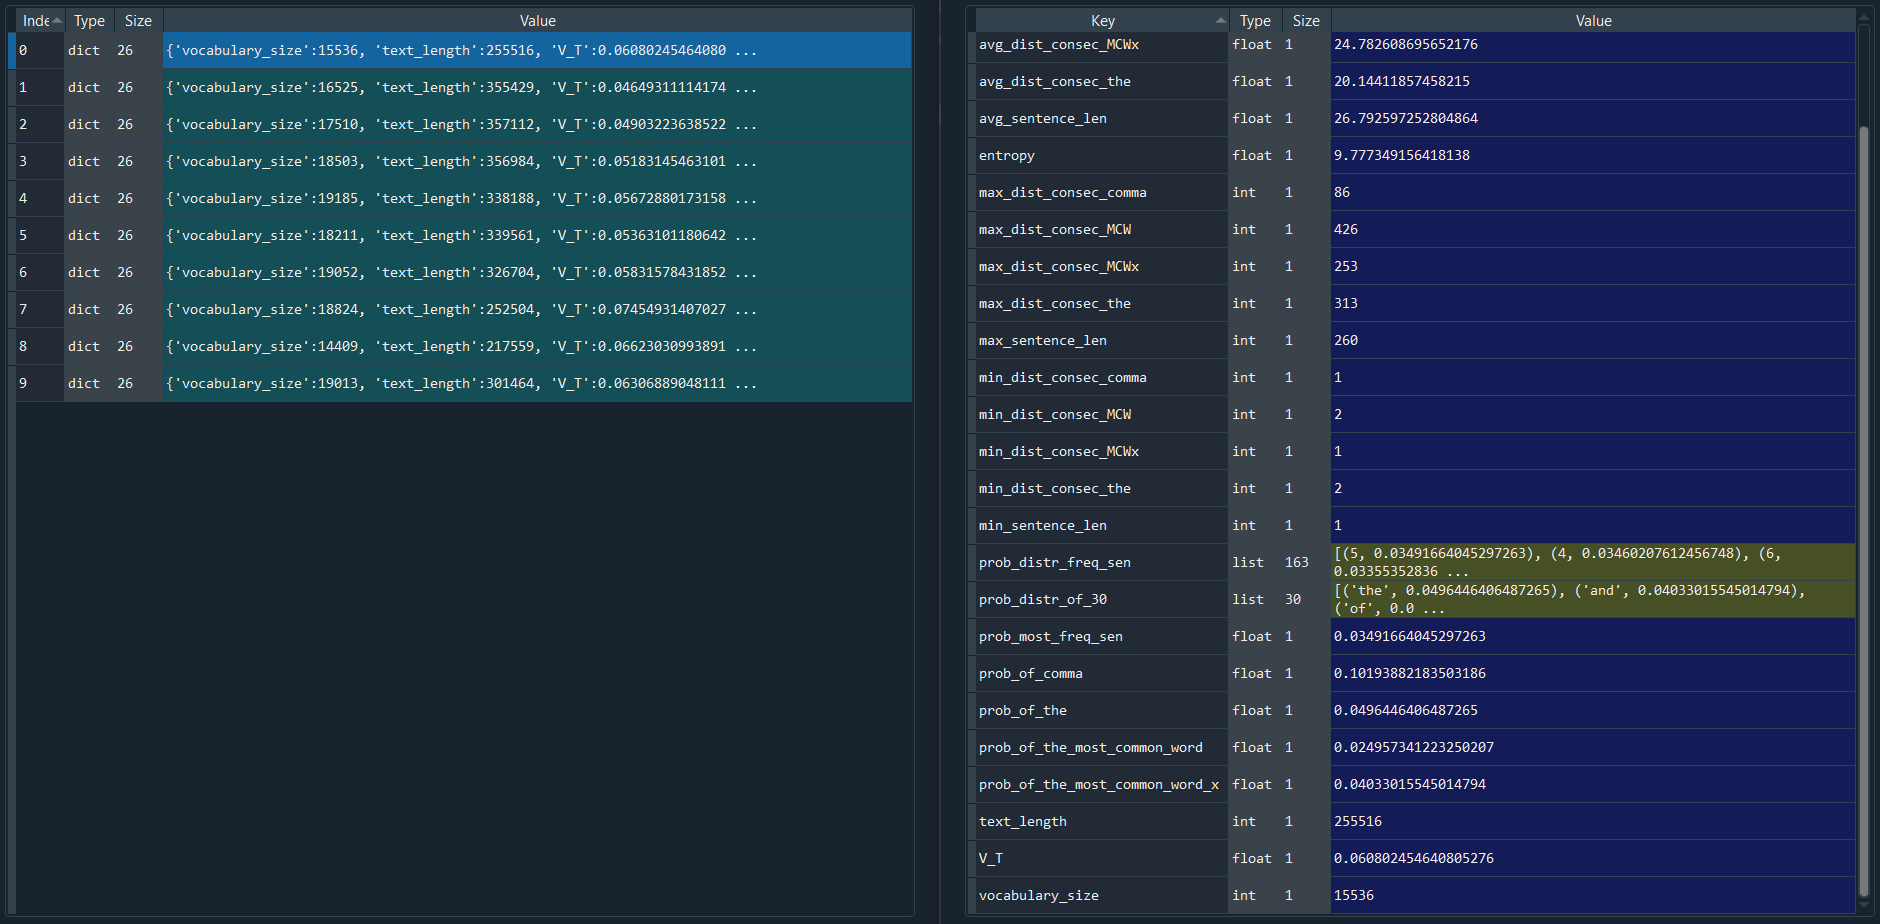
\includegraphics[width=\textwidth, height=\textheight, keepaspectratio]{metriche.png}
\end{figure}

\subsection{Tempistiche al variare dell'input}
Il modulo software che estrae e salva su HDFS le caratteristiche di stile ha impiegato circa 15 minuti per generare i file che contengono le metriche di tutti i testi di ogni autore. Nei nostri test questi ultimi sono 250 e hanno una dimensione totale di 100 MB.

Il modulo software che analizza testi ``sconosciuti'', invece, ha impiegato circa 5 minuti per la generazione dei dizionari delle metriche e la loro successiva classificazione con la stampa a video dei risultati. Nei nostri test sono stati considerati 100 scritti (50 di autori già noti e 50 di autori completamente sconosciuti) per una dimensione totale di 37 MB.

Riportiamo nella seguente tabella il tempo impiegato dai due moduli per produrre il risultato al variare della grandezza dell'input.

\begin{table}[htp]
\centering
\begin{tabular}{ccc}
    \toprule
    \makecell{\textbf{DIMENSIONE} \\ \textbf{INPUT}} & \makecell{\textbf{AGGIUNTA TESTI} \\ \textbf{CONOSCIUTI}} & \makecell{\textbf{CLASSIFICAZIONE} \\ \textbf{TESTI}} \\
    
    \midrule
    1 & 00:12.99 & 00:30.94 \\
    
    \midrule
    2 & 00:15.56 & 00:32.70 \\
    
    \midrule
    3 & 00:17.87 & 00:33.66 \\
    
    \midrule
    4 & 00:20.73 & 00:39.72 \\
    
    \midrule
    5 & 00:24.70 & 00:41.21 \\
    
    \midrule
    10 & 00:36.26 & 00:54.63 \\
    
    \midrule
    15 & 01:17.31 & 01:02.62 \\
    
    \midrule
    25 & 01:41.12 & 01:28.17 \\
    
    \midrule
    50 & 02:37.53 & 02:49.79 \\
    
    \midrule
    100 & 05:24.44 & 05:34.41 \\
    
    \midrule
    250 & 14:51.00 & \texttt{--}:\texttt{--}.\texttt{--} \\
    
    \bottomrule
\end{tabular}
\caption{Performance (mm:ss.ff) al variare della taglia dell'input}
\end{table}

\begin{center}
    \begin{tikzpicture}[scale=1.3]
    \begin{axis}[
    legend pos=north west,
    title style={align=center}, title={Tempo impiegato per l'aggiunta di testi \\ rispetto alla taglia dell'input},
    xlabel={$|input|$},
    ylabel={$tempo \ [min]$},
    xmin=0, xmax=250,
    ymin=0, ymax=15,
    %y label style={font=\tiny},
    %x label style={font=\tiny}
    ]
    
    \addplot[
        color=blue,
        mark=square,
        ]
        coordinates {
            (1,0.2165)(2,0.2593)(3,0.2978)(4,0.3455)(5,0.4117)(10,0.6043)(15,1.2885)(25,1.6853)(50,2.6255)(100,5.4073)(250,14.85)
        };
        \addlegendentry{$curva \ reale$}
    
    \addplot[
        color=red,
        mark=square,
        ]
        coordinates {
            (0,0)(250,15)
        };
        \addlegendentry{$curva \ appros. \ y=0.06x$}
    
    \end{axis}
    \end{tikzpicture}
\end{center}

\begin{center}
    \begin{tikzpicture}[scale=1.3]
    \begin{axis}[
    legend pos=north west,
    title style={align=center}, title={Tempo impiegato per la classificazione \\ rispetto alla taglia dell'input},
    xlabel={$|input|$},
    ylabel={$tempo \ [min]$},
    xmin=0, xmax=100,
    ymin=0, ymax=7,
    %y label style={font=\tiny},
    %x label style={font=\tiny}
    ]
    
    \addplot[
        color=blue,
        mark=square,
        ]
        coordinates {
            (1,0.5157)(2,0.545)(3,0.561)(4,0.662)(5,0.6868)(10,0.9105)(15,1.0437)(25,1.4695)(50,2.8298)(100,5.5735)
        };
        \addlegendentry{$curva \ reale$}
    
    \addplot[
        color=red,
        mark=square,
        ]
        coordinates {
            (0,0)(100,6.07)
        };
        \addlegendentry{$curva \ appros. \ y=0.061x$}
    
    \end{axis}
    \end{tikzpicture}
\end{center}

\subsection{Considerazioni sulle performance}
In realtà Spark potrebbe anche girare in un \textit{ambiente non parallelo}. Infatti, nel caso in cui si volesse operare su un singolo nodo, sarebbe possibile effettuare in maniera più efficiente certe operazioni ma non sarebbe tuttavia possibile distribuire l'elaborazione. Valgono quindi le seguenti considerazioni:
\begin{itemize}
    \item Apache Spark è un framework complesso progettato per distribuire l'elaborazione su centinaia di nodi, garantendo al contempo correttezza e tolleranza agli errori; garantire queste proprietà ha però un costo significativo.
    \item Le operazioni di input/output che Spark svolge su disco e/o in rete sono di ordini di grandezza più lente rispetto all'elaborazione svolta puramente in memoria.
    \item Il parallelismo e l'elaborazione distribuita aggiungono un sovraccarico significativo anche con un carico di lavoro parallelo progettato in maniera ottimale.
    \item Spark dovrebbe essere usato in modalità locale solamente quando si vogliono effettuare dei test, in tal caso infatti non si bada molto alle performance.
\end{itemize}

\subsection{Considerazioni finali}
Ripercorriamo infine quanto abbiamo descritto e osservato in questo documento analizzandolo sezione per sezione:
\begin{itemize}
    \item Nella \hyperref[sec:1]{\textit{sezione 1}} abbiamo introdotto i Big Data e spiegato lo scopo e l'idea alla base di questo progetto.
    \item Nella \hyperref[sec:2]{\textit{sezione 2}} abbiamo analizzato i vantaggi di Spark rispetto a Map-Reduce; in particolare, la scelta di utilizzare Spark è stata dovuta principalmente alla sua maggiore velocità nell'eseguire algoritmi per la manipolazione di dati distribuiti rispetto a Map-Reduce (soprattutto grazie ai diversi tipi di elaborazione e di operatori supportati).
    \item Nella \hyperref[sec:3]{\textit{sezione 3}} abbiamo illustrato la struttura del progetto definendo gli attributi utilizzati per rappresentare lo spazio stilistico di un autore e come questi vengono calcolati dalle funzioni Python implementate; in particolare, abbiamo cercato di far lavorare il codice il più possibile in parallelo per poter garantire un funzionamento efficiente quando si svolge l'elaborazione in un ambiente distribuito.
    \item Nella \hyperref[sec:4]{\textit{sezione 4}} abbiamo presentato alcuni risultati ottenuti durante i nostri test e abbiamo osservato che l'applicativo è in grado di fornire una classificazione accettabile quando gli vengono passati sia testi di autori noti che testi di autori sconosciuti, sempre presumendo che i punteggi di attribuzione restituiti non possono far altro che migliorare nel momento in cui si allena il sistema con un numero più elevato di testi e autori (in un eventuale ambito reale).
    \item Nella \hyperref[sec:5]{\textit{sezione 5}} vengono fornite le istruzioni che spiegano come fare ad eseguire questo progetto e, in particolare, come predisporre l'ambiente distribuito Cloudera in cui è presente il filesystem HDFS.
    \item Nella \hyperref[sec:6]{\textit{sezione 6}} abbiamo infine mostrato le scelte e le strade intraprese durante lo sviluppo di questo progetto e fatto delle considerazioni più approfondite sulle performance che si possono ottenere lavorando in un ambiente parallelo o meno.
\end{itemize}


\newpage
\section{Riferimenti}
Quanto scritto nell'introduzione e sul confronto tra Map-Reduce e Spark è tratto principalmente da slide e dispense del corso di Big Data. Altre fonti: \href{https://spark.apache.org/docs/latest/}{Spark Programming Guides}, \href{https://spark.apache.org/docs/latest/api/python/index.html}{PySpark Documentation}.
\bigskip

\noindent
Gli attributi utilizzati per definire lo spazio stilistico di un autore sono presi dalla Tabella 1 a pagina 150 di:

\textit{Neme, Antonio \& Pulido, J R G \& Muñoz, Abril \& Hernández, Sergio \& Dey, Teresa. January 2015.} \href{https://www.researchgate.net/publication/265604445_Stylistics_analysis_and_authorship_attribution_algorithms_based_on_self-organizing_maps}{Stylistics analysis and authorship attribution algorithms based on self-organizing maps.} \textit{Neurocomputing 147. 147–159.}
\bigskip

\noindent
Le descrizioni delle funzioni Python sono rielaborazioni delle docstring presenti nei relativi file in: \url{https://github.com/zampierida98/authorship}
\bigskip

\noindent
I libri utilizzati per testare le funzionalità del progetto sono presi dal dataset in: \url{https://web.eecs.umich.edu/~lahiri/gutenberg_dataset.html}

Si tratta di una raccolta di circa 3000 libri in lingua inglese (opportunamente privati di alcune parti considerate inutili) scritti da 142 autori diversi che rappresenta un sottoinsieme del \href{http://www.gutenberg.org/}{Progetto Gutenberg}.

\end{document}